\documentclass{article}
\usepackage[utf8]{inputenc}
\usepackage[spanish, es-tabla]{babel}
\usepackage{amsmath}
\usepackage{amssymb}
\usepackage{mathtools}
\usepackage{graphics}
\usepackage{graphicx}
\usepackage{subcaption}

\title{Control Sistemas Mecatrónicos}
\author{BMJIvan }

\begin{document}

\maketitle

%UNIDAD I
%Solución de ecuaciones en espacio de estado
\section{Conceptos fundamentales}

\[
    \text{Aplicaciones}
    \left\{
        \begin{array}{l}
            \text{Transporte de fluidos} \\
            \text{Conversión de la energía} \\
            \text{Acondicionamiento de ambiente} \\
            \text{Turbomáquinaria} \\
            \text{Transporte (vehicular)} 
        \end{array}
    \right.
\]

\[
    \begin{array}{c}
         \text{Áreas de}  \\
         \text{mecánica de fluidos}
    \end{array}
    \left\{ 
        \begin{array}{l}
             \text{Aerodinámica} \\
             \text{Hidráulica} \\ 
             \text{Hidrología} \\
             \text{Metrología}
        \end{array}
    \right.    
    \begin{array}{l}
        \\
        \left\{
            \begin{array}{l}
                \text{Hidráulica de potencia} \\
                \text{Redes de tubería} \\
                \text{Neumática}
            \end{array}
        \right. \\
        \\
        \\
    \end{array}
\]

\[
    \begin{array}{c}
         \text{Técnicas o}  \\
         \text{métodos o analíticos}
    \end{array}
    \left\{ 
        \begin{array}{l}
             \text{Analíticos} \\
             \text{Experimentales} \\ 
             \text{Computacionales} 
        \end{array}
    \right.    
    \begin{array}{l}
        \left\{
            \begin{array}{l}
                \text{Diferenciales} \\
                \text{Diferenciales} 
            \end{array}
        \right.\\
        \\
        \\
    \end{array}
\]

Presión, esfuerzo normal: Genera deformaciones lineales
\[
    P = \lim \frac{ \Delta F_{n} }{ \Delta A } = \frac{ dF_{n} }{ dA }
\]

Esfuerzo cortante: Genera deformaciones angulares 
\[
    \tau = \lim \frac{ \Delta F_{t} }{ \Delta A } = \frac{ dF_{t} }{ dA }
\]

\subsection{Propiedades de los fluidos}
Densidad 
\[ 
    \rho = \frac{ m }{ v } \;\; \Big[ {}^{ kg }/_{ m^3 }. {}^{ lbm }/_{ pie^3 }, {}^{ slug }/_{ pie^3 } \Big]
\]

Peso especifico
\[
    \gamma = \frac{ W_{g} }{ v } = \frac{ mg }{ v } = \rho g \;\; \Big[ {}^{ N }/_{ m^3 }, {}^{ lb }/_{ pie^3 } \Big]
\]

Densidad relativa 
\[
    sg = GE = \rho_{r} = \frac{ \rho_{fluido} }{ \rho_{H_{2}O \;\; T = 4^{o}C} }
\]

Viscosidad dinámica o absoluta
\[
    \mu = \frac{ \tau }{{}^{ d \Vec{u} }/{ dy }} \;\; \frac{ \text{Esfuerzo cortante} }{ \text{Gradiente de velocidad} }
\]
\[
    \mu = \frac{ \tau y }{ \Vec{u} } \;\; \Big[ {}^{N \cdot s }/{ m^{2}, {}^{ lb \cdot s }/{ pie^2 } } \Big]
\]

Viscosidad cinemática
\[
    \nu = \frac{ \mu }{ \rho } \;\; \Big[ {}^{ m^{2} }/{ s }, {}^{ pie^{2} }/{ s } \Big]
\]

\subsection{Gases ideales}

Proceso adiabático: Aquel proceso en el que no se gana ni pierde calor, es decir, cuenta con un aislamiento térmico. 

En proceso adiabático reversible no hay transferencia de calor y por lo tanto el proceso es isoentrópico.

Un proceso adiabático irreversible no es isoentropico. 
\[
    \begin{split}
        \forall & : \text{ Volumen} \\
        \nu & : \text{ volumen especifico \( \frac{ \forall }{ m } = \frac{ 1 }{ \rho } \)}
    \end{split}
\]

\begin{enumerate}
    \item Ley de Boyle y Mariotte
        \[
            \begin{split}
                \text{Si }T & = constante \\
                P \; & \alpha \; \frac{ 1 }{ \forall } \\
                P \forall & = C \\
                P_{ 1 } \forall_{ 1 } & = P_{ 2 } \forall_{ 2 }  
            \end{split}
        \]
    \item Ley de Charles
        \[
            \begin{split}
                \text{Si }P & = constante \\
                \forall\; & \alpha \; T \\
                \frac{ \forall }{ T } & = C \\
                \frac{ \forall_{1} }{ T_{1} } & = \frac{ \forall_{2} }{ T_{2} } 
            \end{split}
        \]
    \item Ley de Gay - Lussac
        \[
            \begin{split}
                \text{Si } \forall & = constante \\
                P \; & \alpha \; T \\
                \frac{ P }{ T } & = C \\
                \frac{ P_{1} }{ T_{1} } & = \frac{ P_{2} }{ T_{2} } 
            \end{split}
        \]
    \item 
        \[
            \begin{split}
                \frac{ P \forall }{ T } & = C \\
                \frac{ P_{1} \forall_{1} }{ T_{1} } & = \frac{ P_{2} \forall_{2} }{ T_{2} } \\
                \frac{ P \nu }{ T } & = nR_{u} \\
                R_{u} & = \frac{ P \forall }{ Tn }
            \end{split}
        \]
        Donde 
        \[
            \begin{split}
                P & = 1 \text{ atmósfera} \\
                T & = 0^{o}C = 273.15K \\
                n & = 1 \text{ kmol} \\
                \forall & = 22.413 m^{3} \\
                R_{u} & = 8.314 {}^{kJ}/_{kmol \cdot K} \\
                n & = \frac{ m }{ M } \; \frac{ \text{ masa } }{ \text{ masa molar } } \\
                R & = \frac{ R_{u} }{ M } \text{ constante del gas }
            \end{split}
        \]
        Entonces 
        \[
            \begin{split}
                R_{u} & = \frac{ P \forall }{ T {}^{m}/{M} } = \frac{ MP \forall }{ Tm } \\
                m \frac{ R_{u} }{ M } & = \frac{ P \forall }{ T } \\
                \frac{ P \forall }{ T } & = mR \\
                P \forall & = TmR \\
                P \frac{ \forall }{ m } & = TR \\
                P \nu & = TR \\
                P & = \frac{ 1 }{ \nu } TR = \rho TR \\
                \frac{ P }{ \rho } & = TR
            \end{split}
        \]
\end{enumerate}

\subsection{ Velocidad sonica o acústica }

A partir de 1
\[
    dp \; \alpha \; - \frac{ d \forall }{ \forall } \\
    dp = -E_{v} \frac{ d \forall }{ \forall }
\]

Donde \( E_{v} \) es el modulo de compresibilidad o modulo volumétrico. \\ 
De la definición de masa
\[
    \begin{split}
        m & = \rho \forall \\
        dm & = \rho dv + d\rho \forall, \;\; dm = 0 \\
        -\rho d\forall & = d\rho \forall \\
        - \frac{ d \forall }{ \forall } & = \frac{ d\rho }{ \rho }
    \end{split}
\]

por lo tanto
\[
    dp = E_{v} \frac{ d\rho }{ \rho }
\]

\[
    C = \sqrt{ \frac{ dp }{ d\rho } } = \sqrt{ \frac{ E_{v} }{ \rho } } \;\; \text{Velocidad del sonido a través de líquidos}
\]
\[
    \begin{split}
        K & = \frac{ C_{p} }{ C_{\nu} } = 1.4 \\
        R & = C_{p} - C_{ \nu } \;\; \Big[ {}^{kJ}/{ kg \cdot K } \Big] \\
        R & = .287 {}^{kJ}/{ kg \cdot K } \\
        C & = \sqrt{ \frac{ k_{p} }{ \rho } } = \sqrt{KTR} \\
        E_{v} & = P \; \text{ Proceso isotérmico} \\
        E_{v} & = KP \; \text{ Proceso isoentropico} \\
    \end{split}
\]
Líquidos incompresibles \( \rho = constante \) \\
Líquidos compresibles \( \rho \not = constante \) 
\[
    \begin{split}
        \text{Mach } & = \frac{ \Vec{v} }{ C } \; \frac{ \text{velocidad fluido} }{ \text{ velocidad de sonido } } \\
        \text{Mach } & \leq .3 \; \text{flujo de gas incompresible} \\
        \text{Mach } & \geq .3 \; \text{flujo compresible}
    \end{split}
\]

\[
    \overbrace{ \frac{ \mu }{ \rho } }^{ \text{Dinámica} } = \overbrace{ v }^{ \text{Cinemática} }
\]

\[
    \begin{split}
        \mu & = \text{ constante o \( 0 \) ideal o no viscoso} \\
        \mu & \not = \text{ constante o \( 0 \) real o viscoso }
    \end{split}
\]

\[
    \begin{array}{c}
         \text{Fluido de acuerdo}  \\
         \text{al comportamiento} \\
         \text{de la \( \mu \)}
    \end{array}
    \left\{ 
        \begin{array}{l}
             \text{Newtoniano} 
                \left\{
                    \begin{array}{l}
                        \tau \; \alpha \; \frac{ d\theta \text{ deformación} }{ dt } \to 
                            \begin{array}{l}
                                \text{ley de viscosidad} \\
                                \text{de Newton}
                            \end{array}
                    \end{array}
                 \frac{ d\theta }{ dt } = \frac{ d\Vec{v} }{ dy } 
                 \right.\\ 
             \text{No Newtoniano} 
                \left\{
                    \begin{array}{l}
                         \tau \text{ no } \; \alpha \; \frac{ d\theta }{ dt } \to \text{ Series de potencias }
                    \end{array}
                \right.\\ 
             \text{Visco-elástico} 
                \left\{
                    \begin{array}{l}
                         \text{Comportamiento Newtoniano}  \\
                         \text{y no Newtoniano}
                    \end{array}
                \right.
        \end{array}
    \right.    
\]

Número de Raynolds
\[
    NR_{E} = \frac{ \text{Fuerzas de inercia} }{ \text{Fuerzas viscosas} } = \overbrace{ \frac{ \rho \Vec{v} D }{ \mu } }^{ \text{Dinámica} } = \overbrace{ \frac{ \Vec{v}D }{ \forall } }^{ \text{Cinemática} }
\]

\[
    \begin{array}{c}
         \text{Flujo viscoso}
    \end{array}
    \left\{ 
        \begin{array}{l}
             \text{flujo laminar} 
                \left\{
                    \begin{array}{l}
                        NR_{E} \leq 2000 \;\; (2300) 
                    \end{array}
                 \right.\\ 
             \text{flujo transición} 
                \left\{
                    \begin{array}{l}
                         2000 \leq NR_{E} \leq 4000
                            \begin{array}{l}
                                \text{puede ser}\\
                                \text{laminar o turbulento}
                            \end{array}
                    \end{array}
                \right.\\ 
             \text{flujo turbulento} 
                \left\{
                    \begin{array}{l}
                         NR_{E} \geq 4000
                    \end{array}
                \right.
        \end{array}
    \right.    
\]

%Transformación de similitud
\subsection{Transformación de similitud}
Considere el vector \( q:n \times 1\;(q\in R^n) \). El conjunto de vectores \( q_{1}, \ldots, q_{m} \) es linealmente dependiente si existen números reales \( \alpha_{1}, \ldots, \alpha_{m} \) no todos cero, tales que
\[
    \alpha_{1}q_{1} + \alpha_{1}q_{1} \ldots, \alpha_{n}q_{n} = 0 \;\; (1)
\]

Si la solución única de (1) es \( \alpha_{1}=\alpha_{2} \ldots =\alpha_{m} \) entonces el conjunto de vectores es linealmente independientes.

A la expresión \( \alpha_{1}q_{1}+\alpha_{2}q_{2}+ \ldots +\alpha_{n}q_{n} \) se le denomina combinación lineal.

Base: Un conjunto de vectores linealmente independientes en \( R^n \) se define como una base si se puede expresar como una combinación lineal única.

En \( R^n \) todo conjunto de vectores linealmente independientes puede utilizarse como una base.

Sea \( X:n \times 1 \) todo vector \( X \) puede expresarse como 
\[
    X=\alpha_{1}q_{1}+ \ldots\ +\alpha_{n}q_{n} \;\; (2)
\] 
donde \( q_{i} \) son linealmente independientes.

De (2) se tiene que
\[
    X=
    \underbrace{
        \begin{bmatrix}
            q_{1},& q_{2},& \ldots,& q_{n}
        \end{bmatrix}
                }_{n \times n}
    \underbrace{
        \begin{bmatrix}
            \alpha_{1} \\
            \alpha_{2} \\
            \vdots \\
            \alpha_{n}
        \end{bmatrix}
                }_{n\times 1} \;\; (3)
\]

Se definen
\[
    Q=
    \begin{bmatrix}
        q_{1},& q_{2},& \ldots,& q_{n}
    \end{bmatrix},\;\;
    \tilde{X}=
    \begin{bmatrix}
        \alpha_{1} \\
        \alpha_{2} \\
        \vdots \\
        \alpha_{n}
    \end{bmatrix}
\]

entonces sustituyendo en (3) se tiene que
\[
    X=Q\tilde{X}
\]

donde \( X \) y \( \tilde{X} \) son similares.

De (2) \( X^\top = \alpha_{1}S_{1} + \alpha_{2}S_{2} + \ldots + \alpha_{n}S_{n}\;\; S_{i}:1\times n \)

\[
    X^\top = 
        \begin{bmatrix}
            \alpha_{1}, & \alpha_{2}, & \ldots & \alpha_{n}
        \end{bmatrix}
        \begin{bmatrix}
            S_{1} \\
            S_{2} \\
            \vdots \\
            S_{n}
        \end{bmatrix}
\]

Una matriz es estable cuando los valores propios son negativos.

Sea la ecuación lineal 
\[
    Ax=y \;\; (4)
\]

donde \( A:n\times n\;\; B:n\times 1\;\; y:n\times 1 \).
se definen
\[
    x=Q\tilde{x}, \;\; y=Q\tilde{y}
\]

Sustituyendo en (4) se tiene que 
\[
    \begin{split}
        AQ\tilde{x} & = Q\tilde{y} \\
        Q^{-1}AQ\tilde{x} & =\tilde{y} \;\; (5)
    \end{split}
\]

donde \( A \) y \( Q^{-1}AQ \) son similares y \(A\) esta relacionada con la estabilidad.

Ejercicio: Sea \( A:n\times n \) una matriz estable, demuestre que la matriz \( \tilde{A} = Q^{-1}AQ \) es también estable, considere que \( Q \) es invertible.

Si
\[
    \begin{split}
        det( \lambda I-A ) & = \lambda^n + alpha_{1}\lambda^{n-1} + \alpha_{2}\lambda^{n-2} + \ldots + \alpha_{n} = 0 \\
        det( \lambda I-\tilde{A} ) & = \lambda^n + alpha_{1}\lambda^{n-1} + \alpha_{2}\lambda^{n-2} + \ldots + \alpha_{n} = 0
    \end{split}
\]

entonces
\[
    \begin{split}
        det( \lambda I-\tilde{A} ) & = det( \lambda I-A ) \\
        det( \lambda I-\tilde{A} ) & = det( \lambda Q^{-1}Q-Q^{-1}AQ )\\
        & = det( Q^{-1}\lambda Q-Q^{-1}AQ ) \\
        & = det( Q^{-1}( \lambda I-A )Q ) \\
        & = det( Q^{-1} ) det( \lambda I-A ) det(Q) \\
        & = det( Q^{-1} ) det(Q) det( \lambda I-A ) \\
        & = det( Q^{-1}Q ) det( \lambda I-A ) \\
        & = det( \lambda I-A )
    \end{split}
\]

repetir el ejercicio anterior considerando la siguiente matriz \(\tilde{A}=QAQ^{-1}\)
\[
    \begin{split}
        det( \lambda I-\tilde{A} ) & = det(\lambda I-A ) \\
        det( \lambda I-A ) & = det( \lambda I-QAQ^{-1} ) \\
        & = det( \lambda QQ^{-1}-QAQ^{-1} ) \\
        & = det( Q\lambda Q^{-1}-QAQ^{-1} ) \\
        & = det( Q( \lambda I-A )Q^{-1} ) \\
        & = det( Q) det( \lambda I-A ) det( Q^{-1} ) \\
        & = det( Q) det( Q^{-1} ) det( \lambda I-A ) \\
        & = det( QQ^{-1} ) det( \lambda I-A ) \\
        & = det( \lambda I-A )
    \end{split}
\]

%Controlabilidad y observabilidad de sistemas lineales
\section{HRM}

\begin{enumerate}
    \item Recursos humanos.
    \begin{itemize}
        \item Capacidades
        \item Habilidades 
        \item Aparición
        \item Horarios
        \item Disponibilidad
    \end{itemize}
    
    \item WBS-EDT estructura y descomposición del trabajo.
    
    \item Asignación de recursos humanos.
\end{enumerate}

Producto: Cualquier cosa que puede ser ofrecida al mercado para satisfacer una necesidad. 

\begin{itemize}
    \item Artesanal
    \item Industrial
\end{itemize}

Exactitud: Cuan cerca del valor real se encuentra el valor medido.

Precisión: Cae en un rango de valores, entre menor sea el rango de valores, mayor será la precisión. 

Proceso: Secuencia de pasos lógicos para obtener un resultado. 

\subsection{EDT-WBS: Estructura del trabajo (Gantt)}

\begin{enumerate}
    \item Definir las actividades: alcance \( \to \) entregables.
    \begin{itemize}
        \item Metodología: Proceso sistemático para lograr "algo".
    \end{itemize}
    
    \item Agrupar actividades: Ciclo de vida del proyecto. Cada grupo de actividades asociar un entregable. 
    
    \item Asignar tiempo, tiempo limites. 
    
    \item Asignar recursos humanos (HRM)
    
    \item Asignar recursos monetarios y recursos materiales. 
\end{enumerate}

%Solución de ecuacines de estado
\subsection{Solución de ecuaciones en espacio de estado 2}

Se condidera el sistema
\[
    (1)
    \left\{
        \begin{array}{lll}
            \dot{x}(t) = Ax(t) + Bu(t)\\
            y(t) = Cx(t) \;\;\;\;x(0)=X_{0}
        \end{array}
    \right.
\]

\[
    \begin{split}
        \dot{x}(t) -Ax(t) & = Bu(t)\\
        e^{-At} (\dot{x}(t)-Ax(t)) & = e^{-At}Bu(t)\\
        e^{-At} (\dot{x}(t)) - e^{-At}Ax(t) & = e^{-At}Bu(t)\\
        \int_{0}^{t} \frac{d}{dt} (e^{-A\tau}x(\tau)) & = \int_{0}^{t} Bu(\tau)d\tau\\
        e^{-A\tau}\Big|_a^b & = \int_{0}^{t} e^{-A\tau} Bu(\tau)d\tau\\
        e^{-At}x(t) - e^{0}x(0) & = \int_{0}^{t} e^{-A\tau} Bu(\tau)d\tau\\
        e^{At} (e^{-At}x(t) - e^{0}x(0)) & = e^{At} \Big(\int_{0}^{t} e^{-A\tau} Bu(\tau)d\tau\Big)\\
        x(t) & = e^{At}x(0) + \int_{0}^{t} e^{(t-\tau)}Bu(\tau)d\tau + C\\
    \end{split}
\]
anteriormente se obtuvo
\[
    x(t) = \mathcal{L}^{-1} \{ (sI-A)^{-1} \} x(0) + \mathcal{L}^{-1} \{ (sI-A)^{-1}Bu(s) \}
\]
Por lo tanto
\[
    e^{At} = \mathcal{L}^{-1} \{ (sI-A)^{-1} \}
\]
A continuación se desarrollará los dos terminos un poco mas.

Se considera la matriz exponencial de la siguiente forma 

\[
    \begin{matrix}
        f(t)=e^{At} & f(0)=I
    \end{matrix}
\]

entonces, partiendo de la derivada 

\[
    \begin{split}
        \dot{f(t)} & = Ae^{At} = Af(t)\\
        \mathcal{L} \{ \dot{f(t)} \} & = \mathcal{L} \{ Af(t) \}\\
        sF(s)-AF(s) & = AF(s)\\
        sF(s)-AF(s) & = F(0)\\
        (sI-A)F(s) & = I\\
        (sI-A)^{-1} (sI-A)F(s) & = (sI-A)^{-1}I\\
        F(s) & = (sI-A)^{-1}\\
        \mathcal{L}^{-1} \{ F(s) \} & = \mathcal{L}^{-1} \{ (sI-A)^{-1} \}\\
        F(t) & = \mathcal{L}^{-1} \{ (sI-A)^{-1} \}\\
        e^{At} & = \mathcal{L}^{-1} \{ (sI-A)^{-1} \}
    \end{split}
\]

Por otro lado, considerando la definicion de la convolución

\[
    h(t)=(f*g)(t) = \int_{0}^{t} f(t-\tau)g(\tau)d\tau 
\]

Según el teorema de la covolución. si \( \mathcal{L} \{ f(t) \} y \mathcal{L} \{g(t)\} \) existen para \( s>a\geq 0, \) entonces

\[
    \mathcal{L} \{f* g\} = \mathcal{L} \{ f(t) \} \mathcal{L} \{ g(t) \}=F(s)G(s)
\]

considerando las ecuaciones 
\[
    \begin{matrix}
        f(t)=e^{At}, & g(t)=Bu(t)
    \end{matrix}
\]

Se tiene que 
\[
    \int_{0}^{t} e^{At-\tau} Bu(\tau)d\tau = f*g
\]

Aplicando la transformada de Laplace se tiene que

\[
    \begin{split}
        \mathcal{L} \Big\{ \int_{0}^{t} e^{At-\tau} Bu(\tau)d\tau \Big\} & =\mathcal{L} \Big\{ f*g \Big\}\\
        & = F(s)G(s)\\
        & = (SI-A)^{-1}Bu(s)
    \end{split}
\]

Por lo tanto aplucando la transformada inversa de Laplace se obtiene

\[
    \int_{0}^{t} e^{At-\tau} Bu(\tau)d\tau = \mathcal{L}^{-1} \Big\{ (SI-A)^{-1}Bu(s) \Big\}
\]

%Criterios de controlabilidad y observabilidad
\section{Criterios de estabilidad}

El sistema 
\[
    (1)
    \left\{
        \begin{array}{lll}
            \dot{x}(t) = Ax(t) + Bu(t)\\
            y(t) = Cx(t)
        \end{array}
    \right.
\]

O el par \( (A, B)\) es controlable si cumple alguno de los siguientes criterios.

1) Controlabilidad de Kalman
La matriz de controlabilidad
\[
    C = 
    \begin{bmatrix}
        \underbrace{B}_{n\times m} &
        \underbrace{AB}_{n\times m} &
        A^{2}B & \ldots & A^{n-1}B
    \end{bmatrix}
    \Big\} n\times nm
\]

para \( m=1 \) (una entrada), con \( det(C)\not= 0 \) es de rango completo, es decir, \( rango(C)=n \).

2) Controlabilidad de Hautus
La matriz de controlabilidad
\[
    H =
    \begin{bmatrix}
        \lambda I-A & B
    \end{bmatrix}
    \Big \} n\times(n+m)
\]
es de rango completa, \( rango(HC)=n \) para todo \( \lambda \in \mathbb{C} \)

3) Gramiano de controlabilidad
\[
    G_{c} = \int_{0}^{t} e^{At\tau}BB^{T}e^{A^{T}\tau}d\tau
\]
es invertible, es decir, \( det(G_{c}) \not= 0) \)

4) Los valores propios de la matriz \( A-Bk \) pueden asignarse arbitrariamente.

\section{Criterios de observabilidad}
El sistema 
\[
    (1)
    \left\{
        \begin{array}{lll}
            \dot{x}(t) = Ax(t) + Bu(t)\\
            y(t) = Cx(t)
        \end{array}
    \right.
\]

O el par \( (A, B)\) es observable si cumple alguno de los siguientes criterios.

1) Observabilidad de Kalman
La matriz de observabilidad
\[
    C = 
    \left.
    \begin{bmatrix}
        C \\
        CA \\
        CA^{2} \\ \vdots \\
        CA^{n-1}
    \end{bmatrix}
    \right\} pn\times n
\]

es de rango completo, \( rango(C)=n \).

2)Observabilidad de Hautus
La matriz de observabilidad
\[
    H_{o} =
    \begin{bmatrix}
        \lambda I-A \\ 
        C
    \end{bmatrix}
\]
es de rango completa, \( rango(H_{o})=n \) para todo \( \lambda \in \mathbb{C} \)

3) Gramiano de observabilidad
\[
    G_{o} = \int_{0}^{t} e^{At\tau}C^{T}Ce^{A^{T}\tau}d\tau
\]
es invertible, \( det(G_{o}) \not= 0) \)

4) Los valores propios de la matriz \(A-LC\) pueden asignarse arbitrariamente.

%Forma canónica controlable
\subsection{Forma Canónica Controlable}

Ejercicio: demostrar que la propiedad de controlabilidad es invariante para cualquier transformación de similitud.

Se considera la transformación de similitud
\[
    (1) \;\; X = P^{-1}z
\]

donde \( P \) es invertible
Se toma el sistema 
\[(2)
    \left\{
        \begin{array}{lll}
            \dot{x}(t) = Ax(t) + Bu(t) \\
            y(t) = Cx(t)
        \end{array}
    \right.
\]

Se sustituye (1) en (2) para conseguir \( P^{-1}\dot{z} = AP^{-1}z+Bu \), y así, obtener el sistema
\[(3)
    \left\{
        \begin{array}{lll}
            \dot{z}(t) = \overbrace{ PAP^{-1}}^{\tilde{A} } + \overbrace{ PBu}^{\tilde{B} } \\
            y(t) = CP^{-1}
        \end{array}
    \right.
\]
donde \( A \) y \( PAP^{-1} \) son invariantes, se tiene que \( \lambda (A) = \lambda(PAP^{-1}) \) debido a que \( P \) es invertible, entonces \( rango( \tilde{C} ) = rango(C) \).

Se obtiene la matriz de controlabilidad para los sistemas (2) y (3) respectivamente.
\[(4) \;\;
    C=[B , AB , A^{2}B , \ldots , A^{n-1}B]
\]
\[(5) \;\;
    \tilde{C} = [\tilde{B} , \tilde{A}\tilde{B} , \tilde{A}^{2}\tilde{B} , \ldots , \tilde{A}^{n-1}\tilde{B}]
\]

Considerando que \( (PAP^{-1})^{n} = PA^{n}P^{-1} \), se sustituye las matrices similares de (3) en (5)
\[
    \begin{split}
        \tilde{C} & = [PB, PAP^{-1}PB, PA^{2}P^{-1}PB, \ldots, PA^{n-1}P^{-1}PB] \\
        \tilde{C} & = P[B, AB, A^{2}B, \ldots, A^{n-1}B] \\
        \tilde{C} & = PC 
    \end{split}
\]

Lo que se busca es la matriz \( P \), por lo tanto, de la ecuación anterior se puede despejar de la siguiente forma
\[
    \begin{split}
        \tilde{C} & = PC \\
        \tilde{C}\tilde{C}^{-1} & = PC\tilde{C}^{-1} \\
        I & = PC\tilde{C}^{-1} \\
        P^{-1}I & = C\tilde{C}^{-1} \\
        P^{-1} & = C\tilde{C}^{-1} \;\; (6)
    \end{split}
\]

Ahora se tomará el sistema de entradas y salidas
\[
    \begin{split}
        y^{n}(t) + a_{1}y^{n-1}(t) + \ldots + a_{n}y(t) & = b_{1}u^{n-1}(t) + \ldots + b_{n}u(t) \\
        \mathcal{L} \{ y^{n}(t) + a_{1}y^{n-1}(t) + \ldots + a_{n}y(t) \} & = \mathcal{L} \{ b_{1}u^{n-1}(t) + \ldots + b_{n}u(t) \} \\
        y(s)s^{n} + a_{1}y(s)s^{n-1} + \ldots + a_{n}y(s) & = b_{1}u(s)s^{n-1} + \ldots + b_{n}u(s) \\
        y(s) (s^{n} + a_{1}s^{n-1} +\ldots + a_{n} ) & = u(s) (b_{1}s^{n-1} + \ldots + b_{n})
    \end{split}
\]

Se escribe la función de transferencia como 
\[
    g(s) = \frac{y(s)}{u(s)} = \frac{ b_{1}s^{n-1} + \ldots + b_{n} }{ s^{n} + a_{1}s^{n-1} +\ldots + a_{n} } = \frac{N(s)}{D(s)}
\]

Si consideramos una función de transferencia racional (sin retardo) y estrictamente propia (orden del denominador mayor que el numerador)
\[
    g(s)=N(s)D(s)^{-1}
\]
donde N(s) y D(s) son polinomios. Por lo tanto, la función de transferencia se puede escribir como 
\[
    g(s) = \frac{y(s)}{u(s)} = N(s)D(s)^{-1}
\]

La salida del sistema se puede escribir como 
\[
    y(s) = N(s)D(s)^{-1}u(s)
\]

donde \( v(s) = D(s)^{-1}u(s) \). Entonces la entrada y la salida se pueden escribir como 
\[
    \begin{split}
        u(s) & = D(s)v(s) \\
        y(s) & = N(s)v(s)
    \end{split}
\]

Se definen las variables de estado de la siguiente forma
\[ 
    \begin{bmatrix}
        X_{1}(s) \\
        X_{2}(s) \\
        \vdots \\
        X_{n-1}(s) \\
        X_{n}(s)
    \end{bmatrix}
    =
    \begin{bmatrix}
        S^{n-1} \\
        S^{n-2} \\
        \vdots \\
        S \\
        1
    \end{bmatrix} v(s)
\]

entonces las variables de estado se pueden escribir como
\[
    \begin{split}
        X_{n} & = v(s) \\
        X_{n-1} = sv(s) & = sX_{n}(s) \\
        X_{n-2}(s) = S^{2}v(s) =s(sv(s)) & = sX_{n-1}(s) \\
        &\;\;\vdots \\
        X_{2}(s) & = sX_{3}(s) \\
        X_{1}(s) & = sX_{2}(s)
    \end{split}
\]

Si se sustituyen las variables de estado en la entrada se obtiene lo siguiente
\[
    u(s) = sX_{1}(s) + a_{1}X_{1}(s) + \ldots + a_{n}X_{n}(s)
\]

Se despeja \( sX_{1}(s) \)
\[
    sX_{1}(s) = -a_{1}X_{1}(s) - \ldots - a_{n}X_{n} + u(s)
\]

Entonces es posible escribir el espacio de estados como
\[
    \begin{bmatrix}
        SX_{1}(s) \\
        SX_{2}(s) \\
        \vdots \\
        SX_{n}(s)
    \end{bmatrix}
    =
    \underbrace{
        \begin{bmatrix}
        -a_{1} & -a_{2} & \cdots & -a_{n} \\
        1 & 0 & \cdots & 0 \\
        \vdots & \ddots & \cdots & \vdots \\
        0 & \cdots & 1 & 0
        \end{bmatrix}
                }_{\tilde{A}}
    \begin{bmatrix}
        X_{1}(s) \\
        X_{2}(s) \\
        \vdots \\
        X_{n}(s)
    \end{bmatrix}
    +
    \underbrace{
        \begin{bmatrix}
            \\ 0 \\ \vdots \\ 0
        \end{bmatrix}
                }_{\tilde{B}}
     u(s)
\]

Según la definición de la matriz similar de controlabilidad
\[
    \tilde{C} = [
    \tilde{B},
    \tilde{A}\tilde{B},
    \tilde{A}^{2}\tilde{B},
    \cdots,
    \tilde{A}^{n-1}\tilde{B} ]
\]

Se usará una matriz de 3*3 para encontrar un patrón
\[
    \tilde{C} = 
    \begin{bmatrix}
        1 & -a_{1} & -a_{1}^{2}-a_{2} \\
        0 & 1 & -a_{1} \\
        0 & 0 & 1
    \end{bmatrix}
\]

La inversa esta dada por
\[
    \tilde{C}^{-1} = 
    \begin{bmatrix}
        1 & a_{1} & a_{2} \\
        0 & 1 & a_{1} \\
        0 & 0 & 1
    \end{bmatrix}
\]

Por lo tanto, la inversa de la matriz similar de controlabilidad se puede expresar como 
\[
    \tilde{C}^{-1} = 
    \begin{bmatrix}
        1 & a_{1} & a_{2} & \cdots & a_{n-1} \\
        0 & 1 & a_{1} & \cdots & a_{n-2} \\
        \vdots & \ddots & \ddots & \ddots & \vdots \\
        0 & 0 & 0 & \ddots & a_{1} \\
        0 & 0 & 0 & \cdots & 1
    \end{bmatrix}
\]

Considerando la matriz de controlabilidad 
\[
    C = [B, AB, A^{2}B, \cdots, A^{n-1}B ]
\]

La ecuación (6) se puede escribir como
\[
    P^{-1} =
    [B, AB, A^{2}B, \cdots, A^{n-1}B ]
    \begin{bmatrix}
        1 & a_{1} & a_{2} & \cdots & a_{n-1} \\
        0 & 1 & a_{1} & \cdots & a_{n-2} \\
        \vdots & \ddots & \ddots & \ddots & \vdots \\
        0 & 0 & 0 & \ddots & a_{1} \\
        0 & 0 & 0 & \cdots & 1
    \end{bmatrix}
\]

%Forma canónica observable
\subsection{Forma Canonica Observable}
Ejercicio: Demostrar que la propiedad de observabilidad es invariante para cualquier transformación de similitud.

Se considera la transformación de similitud
\[
    (1)\:\:
    x = Qz
\]

donde Q es invertible. Se toma el sistema
\[
    (2)
    \left\{
        \begin{array}{lll}
            \dot{x}(t) = Ax(t) + Bu(t)\\
            y(t) = Cx(t)
        \end{array}
    \right.
\]

Se sustituye (1) en (2) para obtener \( Q\dot{z} = AQz+Bu \) y asu obtener el sistema
\[
    (3)
    \left\{
        \begin{array}{lll}
            \dot{z}(t) =
                \overbrace{Q^{-1}AQz}^{\tilde{A}}+ 
                \overbrace{Q^{-1}Bu}^{\tilde{B}}\\
            y(t) = \underbrace{
                CQz
            }_{\tilde{C}}
        \end{array}
    \right.
\]

Se obtiene la matriz de observabilidad para los sistemas (2) y (3) respectivamente.
\[
    \begin{split}
        (4)\;\;
        O & =\left[
        \begin{array}{cc}
            C \\
            CA \\
            CA^{2} \\
            \vdots \\
            CA^{n-1}
        \end{array}\right]
        =[C, CA, CA^{2}, \ldots, CA^{n-1}]^{T}
        \\
        (5)\;\;
        \tilde{O} & = \left[
        \begin{array}{cc}
            \tilde{C} \\
            \tilde{C}\tilde{A} \\
            \tilde{C}\tilde{A}^{2} \\
            \vdots \\
            \tilde{C}\tilde{A}^{n-1}
        \end{array}\right]
        =[\tilde{C}, \tilde{C}\tilde{A}, \tilde{C}\tilde{A}^{2}, \ldots, \tilde{C}\tilde{A}^{n-1}]^{T}
    \end{split}
\]

Debido a que \( \tilde{A}^{n} = Q^{-1}\tilde{A}^{n}Q \)
\[
    \begin{split}
        \tilde{O} & = [CQ, CQQ^{-1}AQ, CQQ^{-1}A^{2}Q, \ldots, CQQ^{-1}A^{n-1}Q]^{T}\\
        \tilde{O} & = [CQ, CAQ, CA^{2}Q, \ldots, CA^{n-1}Q]^{T}\\
        \tilde{O} & = [C, CA, CA^{2}, \ldots, CA^{n-1}]^{T}Q\\
        \tilde{O} & = OQ 
    \end{split}
\]

Lo que se busca es la matriz Q, por lo tanto, de la ecuación anterior se puede despejar de la siguiente forma
\[
    \begin{split}
        \tilde{O} & = OQ \\
        \tilde{O}Q^{-1} & = OQQ^{-1} \\
        \tilde{O}Q^{-1} & = OI \\
        \tilde{O}^{-1}\tilde{O}Q^{-1} & = \tilde{O}^{-1}O\\
        IQ^{-1} & = \tilde{O}^{-1}O\\
        Q^{-1} & = \tilde{O}^{-1}O \;\;(6)
    \end{split}
\]

Debido a que \( Q \) es invertible, \( rango(\tilde{O}) = rango(O)\) 

Tomando el sistema de entradas salidas
\[
    y(s)s^{n} + a_{1}y(s)s^{n-1} + \ldots + a_{n}y(s) = b_{1}u(s)s^{n-1} + \ldots + b_{n}u(s) \;\;(7)
\]

Se reacomoda de la siguiente forma
\[
    s^{n}y(s) + s^{n-1}(a_{1}y(s)-b_{1}u(s)) + \ldots + s(a_{n-1}y(s)-b_{n-1}u(s)) = b_{n}u(s)-a_{n}y(s) 
\]

Se considera la variable de estado \( X_{n}(s) = y(s) \), es decir
\[
    y(s) = [0,0,0,\ldots,1]X(s)
\]

Entonces se comienza a definir las variables de estado a partir de (7), de la siguiente forma
\[
    \begin{split}
        s^{n}y(s) + s^{n-1}(a_{1}y(s)-b_{1}u(s)) 
        + \ldots + s(a_{n-1}y(s)-b_{n-1}u(s)) & = b_{n}u(s)-a_{n}y(s)\\
        s^{n-1}sy(s) + s^{n-1}(a_{1}y(s)-b_{1}u(s)) 
        + \ldots + s(a_{n-1}y(s)-b_{n-1}u(s)) & = b_{n}u(s)-a_{n}y(s)\\
        s^{n-1}(sy(s)+a_{1}y(s)-b_{1}u(s))+ \ldots + s(a_{n-1}y(s)-b_{n-1}u(s)) & = b_{n}u(s)-a_{n}y(s)\\
        s^{n-1}
        \overbrace{(sy(s)+a_{1}y(s)-b_{1}u(s))}^{X_{n-1}(s)} + \ldots + s(a_{n-1}y(s)-b_{n-1}u(s)) & = b_{n}u(s)-a_{n}y(s)\\
        s^{n-1}X_{n-1}(s)+s^{n-2}(a_{2}y(s)-b_{2}u(s)) + \ldots + s(a_{n-1}y(s)-b_{n-1}u(s)) & = b_{n}u(s)-a_{n}y(s)\\
        s^{n-2}sX_{n-1}(s)+s^{n-2}(a_{2}y(s)-b_{2}u(s)) + \ldots + s(a_{n-1}y(s)-b_{n-1}u(s)) & = b_{n}u(s)-a_{n}y(s)\\
        s^{n-2}(sX_{n-1}(s)+(a_{2}y(s)-b_{2}u(s))) + \ldots + s(a_{n-1}y(s)-b_{n-1}u(s)) & = b_{n}u(s)-a_{n}y(s)\\
        s^{n-2}
        \overbrace{(sX_{n-1}+a_{2}y(s)-b_{2}u(s))}^{X_{n-2}(s)} + \ldots + s(a_{n-1}y(s)-b_{n-1}u(s)) & = b_{n}u(s)-a_{n}y(s)\\
    \end{split}
\]
\[
    \;\vdots
\]
\[
    \begin{split}
        s^{2}X_{2}(s)+s(a_{n-1}y(s)-b_{n-1}u(s)) & = b_{n}u(s)-a_{n}y(s)\\
        s
        \overbrace{(sX_{2}(s)+a_{n-1}y(s)-b_{n-1}u(s))}^{X_{1}(s)} & = b_{n}u(s)-a_{n}y(s)\\
        sX_{1}(s) & = b_{n}u(s)-a_{n}y(s)\\
    \end{split}
\]

Por lo tanto las variables de estado se definen como
\[
    \begin{split}
        X_{1}(s) & = sX_{2}(s)+a_{n-1}y(s)-b_{n-1}u(s)\\
        &\vdots\\
        X_{n-2}(s) & = sX_{n-1}(s)+a_{2}y(s)-b_{2}u(s)\\
        X_{n-1}(s) & = sX_{n}(s)+a_{1}y(s)-b_{1}u(s)\\
        X_{n}(s) & = y(s)
    \end{split}
\]

Del proceso para obtener las variables de estado se puede ver que 
\[
    \begin{split}
        sX_{1}(s) & = -a_{n}y(s)+b_{n}u(s)\\
        s^{2}X_{2}(s)+s(a_{n-1}y(s)-b_{n-1}u(s)) & = -a_{n}y(s)+b_{n}u(s)\\
        s^{2}X_{2}(s)+s(a_{n-1}y(s)-b_{n-1}u(s)) & = sX_{1}(s)\\
        sX_{2}(s)+(a_{n-1}y(s)-b_{n-1}u(s)) & = X_{1}(s)\\
        sX_{2}(s) & = X_{1}(s)-a_{n-1}y(s)+b_{n-1}u(s)
    \end{split}
\]

entonces la derivada de las variables de estado se pueden escribir de la siguiente forma
\[
    \begin{split}
        sX_{1}(s) & = -a_{n}y(s)+b_{n}u(s)\\
        sX_{2}(s) & = X_{1}(s)-a_{n-1}y(s)+b_{n-1}u(s)\\
        \vdots\\
        sX_{n-1}(s) & = X_{n-2}(s)-a_{2}y(s)+b_{2}u(s)\\
        sX_{n}(s) & = X_{n-1}(s)-a_{1}y(s)+b_{1}u(s)
    \end{split}
\]

Recordando que \( X_{n}(s) = y(s) \) se tiene que 
\[
    \begin{split}
        sX_{1}(s) & = -a_{n}X_{n}(s)+b_{n}u(s)\\
        sX_{2}(s) & = X_{1}(s)-a_{n-1}X_{n}(s)+b_{n-1}u(s)\\
        \vdots\\
        sX_{n-1}(s) & = X_{n-2}(s)-a_{2}X_{n}(s)+b_{2}u(s)\\
        sX_{n}(s) & = X_{n-1}(s)-a_{1}X_{n}(s)+b_{1}u(s)
    \end{split}
\]

Entonces es posible escribir el espacio de estados como
\[
    \begin{bmatrix}
        SX_{1}(s) \\
        SX_{2}(s) \\
        \vdots \\
        SX_{n}(s)
    \end{bmatrix}
    =
    \underbrace{
        \begin{bmatrix}
        0 & 0 & \cdots & -a_{n}\\
        1 & 0 & \cdots & -a_{n-1} \\
        \vdots & \ddots & \cdots & \vdots \\
        0 & \cdots & 1 & -a_{1}
        \end{bmatrix}
                }_{\tilde{A}}
    \begin{bmatrix}
        X_{1}(s) \\
        X_{2}(s) \\
        \vdots \\
        X_{n}(s)
    \end{bmatrix}
    +
    \underbrace{
        \begin{bmatrix}
        b_{n}\\
        b_{n-1}\\
        \vdots\\
        b_{1}
        \end{bmatrix}
                }_{\tilde{B}}
     u(s)
\]
\[
    y(s) = \underbrace{[0,0,\ldots,1]}_{\tilde{C}}X(s)
\]

Según la definición de la matriz similar de observabilidad
\[
    \tilde{O} = [
    \tilde{C},
    \tilde{C}\tilde{A},
    \tilde{C}\tilde{A}^{2},
    \cdots,
    \tilde{C}\tilde{A}^{n-1} ]^{T}
\]

Se usará una matriz de 3*3 para encontrar un patrón
\[
    \tilde{O} = 
    \begin{bmatrix}
        0 & 0 & 1 \\
        0 & 1 & -a_{1} \\
        0 & -a_{1} & -a_{2}+a_{1}^{2}
    \end{bmatrix}
\]

La inversa esta dada por
\[
    \tilde{C}^{-1} = 
    \begin{bmatrix}
        a_{2} & a_{1} & 1 \\
        a_{1} & 1 & 0 \\
        1 & 0 & 0
    \end{bmatrix}
\]

Por lo tanto, la inversa de la matriz similar de controlabilidad se puede expresar como 
\[
    \tilde{O}^{-1} = 
    \begin{bmatrix}
        a_{n-1} & a_{n-2} & \cdots & a_{1} & 1 \\
        a_{n-2} & a_{n-3} & \cdots & 1 & 0\\
        \vdots & \rotatebox{90}{\(\ddots\)} & \rotatebox{90}{\(\ddots\)} & \vdots & \vdots\\
        a_{1} & 1 & 0 & \cdots & 0\\
        1 & 0 & 0 & \cdots & 0
    \end{bmatrix}
\]

Considerando la matriz de observabilidad 
\[
    O = [C, CA, CA^{2}, \ldots, CA^{n-1}]^{T}
\]

La ecuación (6) se puede escribir como
\[
    Q^{-1} =
    \begin{bmatrix}
    a_{n-1} & a_{n-2} & \cdots & a_{1} & 1 \\
    a_{n-2} & a_{n-3} & \cdots & 1 & 0\\
    \vdots & \rotatebox{90}{\(\ddots\)} & \rotatebox{90}{\(\ddots\)} & \vdots & \vdots\\
    a_{1} & 1 & 0 & \cdots & 0\\
    1 & 0 & 0 & \cdots & 0
    \end{bmatrix}
    \begin{bmatrix}
        C\\
        CA\\
        CA^{2}\\
        \vdots\\
        CA^{n-1}
    \end{bmatrix}
\]

%UNIDAD II
%Diseño de sistemas de control en espacios de estado
\section{Diseño conceptual}
Con base en los sistemas que conforman la arquitectura física se requiere comenzar a buscar posibles soluciones. Estas soluciones deben cumplir las funciones, los requerimientos y las necesidades.

La integración de las soluciones por cada uno de los módulos se denomina diseño conceptual.

\begin{enumerate}
    \item Análisis morfológico, caja morfológica
        \begin{itemize}
            \item De cada característica se requiere al menos una posible solución. 
            \item Posibles soluciones, no importa si parecen "absurdas".
            \item Mayor cantidad de posibles soluciones.
        \end{itemize}
        
        \begin{table}[h]
            \centering
            \begin{tabular}{|c|c|c|c|}
                \hline
                \( C_{1} \) & \( Ps_{11} \) & \( \cdots \)& \( Ps_{1j} \) \\
                \( C_{2} \) & \( Ps_{21} \) & \( \cdots \) & \( Ps_{2j} \) \\
                \( \vdots \) & \( \vdots \) & & \( \vdots \) \\
                \( C_{i} \) & \( Ps_{i1} \) & \( \cdots \) & \( Ps_{ij} \) \\
                \hline
            \end{tabular}
            \caption{Caja morfológica}
        \end{table}
        
        No
        \begin{itemize}
            \item Componentes
            \item Materiales
            \item Procesos de manufactura
        \end{itemize}
        
        Si
        \begin{itemize}
            \item Mecanismos 
            \item Controladores
            \item Formas
            \item Métodos
            \item Ubicación componentes 
        \end{itemize}
        
        \item Generar combinaciones
        \begin{itemize}
            \item Deben ser congruentes
            \item De 3 a 5 combinaciones
            \item Deben incluir todas las características
            \item Deben buscar el mejor desempeño de las funciones
        \end{itemize}
        Cada combinación se denomina "Diseño conceptual"
        
        \item Seleccionar el mejor diseño conceptual
        \begin{itemize}
            \item Generar los criterios de selección
            \item Determinar una herramienta de selección multicriterio 
            \item Resolver el problema de selección
        \end{itemize}
        
        \item Analizar resultados del método de selección
        
        \item Comprobar
\end{enumerate}

%Ubicación de polos método directo
\subsection{Ubicación de polos: método directo}
Considere un sistema SISO
\[(1)
    \left\{
        \begin{array}{lll}
            \dot{x}(t) = Ax(t) + Bu(t) \\
            y(t) = Cx(t)
        \end{array}
    \right.
\]
El polinomio característico de (1)
\[
    \begin{split}
        P(s) & = det(sI-A) = 0\\
        & = s^{n} + a_{1}s^{n-1} + a_{2}s^{n-2} + \ldots + a_{n}\\
        & = (s-q_{1}) (s-q_{2}) \ldots (s-q_{n})
    \end{split}
\]

donde \( q_{1}, q_{2}, \ldots, q_{n} \) son los polos del sistema en lazo abierto.
El problema de ubicación de polos consiste en asignar los polos \( \mu_{1}, \mu_{2}, \ldots, \mu_{n} \) al sistema en lazo cerrado, entonces
\[
    P_{LC} = (s-\mu_{1}) (s-\mu_{2}) \ldots (s-\mu_{n}) = s^{n} + \tilde{a}_{1}s^{n-1} + \tilde{a}_{2}s^{n-2} + \ldots + \tilde{a}_{n}
\]

Es decir, que se encontraran las ganancias que permitan que los polos \( \mu_{1}, \mu_{2}, \ldots, \mu_{n} \) aparezcan en el polinomio característico del sistema en lazo cerrado. Por lo tanto en este punto los polos en lazo cerrado son conocidos.

Se define la retroalimentación de estado
\[
    \begin{split}
        (2) \;\; 
        u & = r - kx \;\; donde \;\; k:1 \times n \\
        & = r - [k_{1}, k_{2}, \ldots, k_{n}]
        \begin{bmatrix}
            x_{1} \\ x_{2}\\ \vdots \\ x_{n}
        \end{bmatrix} \\
        & = r - (k_{1}x_{1} + k_{2}x_{2} + \ldots + k_{n}x_{n}) \\
        & = r - \sum_{i=1}^{n} k_{i}x_{i}
    \end{split}
\]

Sustituyendo (2) en (1)
\[
    \begin{split}
        \dot{x} & = Ax + B(r-kx) \\
        & = Ax + Br -Bkx \\
        & = (A-Bk)x + Br \;\; (3) \text{ sistema en lazo cerrado}
    \end{split}
\]

Por lo tanto el polinomio característico en lazo cerrado es
\[
    \begin{split}
        P_{LC}(s) & = det(sI-(A -Bk)) = 0\\
        & = (s-\mu_{1}) (s-\mu_{2}) \ldots (s-\mu_{n})\\
        & = s^{n} + \tilde{a}_{1}s^{n-1} + \tilde{a}_{2}s^{n-2} + \ldots + \tilde{a}_{n}
    \end{split}
\]

Ejemplo: determinar las ganancias \( k = K_{1}, k_{2} \) para ubicar los polos \( \mu_{1} = -1+j,\; \mu_{2}=-1-j \), considerando el siguiente sistema en lazo abierto
\[
    A =
    \begin{bmatrix}
        1 & 3 \\
        3 & 1 
    \end{bmatrix}, \;\;
    B = 
    \begin{bmatrix}
        1 \\ 0
    \end{bmatrix}
\]

Conociendo los polos, se puede obtener el polinomio característico de la siguiente forma
\[
    \begin{split}
        P_{LC}(s) & = (s-(-1+j)) (s-(-1-j)) \\
        & = (s+1-j) (s+1+j) \\
        & = s^{2} + s + sj + s + 1 + j - sj -j -j^{2} \\
        & = s^{2} + 2s + 2
    \end{split}
\]

Por lo tanto
\[
    \tilde{a}_{1} = 2 \;\; \tilde{a}_{2} = 2
\]

Por otro lado el polinomio característico se calcula usando las matrices \( A \) y \( B \) como 
\[
    \begin{split}
        P_{LC}(s) & = det(sI-(A-Bk)) \\
        & = det
            (s
                \begin{bmatrix} 1 & 0 \\ 0 & 1   \end{bmatrix}
                -(
                \begin{bmatrix} 1 & 3 \\ 3 & 1  \end{bmatrix} 
                - 
                \begin{bmatrix} 1 \\ 0  \end{bmatrix}
                \begin{bmatrix} k_{1} & k_{2}   \end{bmatrix})
            ) \\
        & = det
            (
                \begin{bmatrix} s & 0 \\ 0 & s   \end{bmatrix}
                -
                \begin{bmatrix} 1 & 3 \\ 3 & 1  \end{bmatrix}
                +
                \begin{bmatrix} k_{1} & k_{2} \\ 0 & 0  \end{bmatrix}
            ) \\
        & = det
            (
                \begin{bmatrix} s & 0 \\ 0 & s   \end{bmatrix}
                +
                \begin{bmatrix} k_{1}-1 & k_{2}-3 \\ -3 & -1  \end{bmatrix}
            ) \\
        & = det
            (
            \begin{bmatrix}
                        s+k_{1}-1 & k_{2}-3 \\
                        -3 & s-1 \\
            \end{bmatrix}
            ) \\
        & = s^{2} + sk_{1} - s - s - k_{1} + 1 + 3_{2} - 9 \\
        & = s^{2} + (k_{1} - 2)s + 3k_{2} - k_{1} - 8
    \end{split}
\]

Igualando ambos polinomios característicos, se puede obtener el siguiente sistema de ecuaciones
\[
    \begin{split}
        2 & = k_{1} -2 \\
        2 & = 3k_{2} - k_{1} - 8
    \end{split}
\]

Resolviendo el sistema de ecuaciones se obtienen las ganancias para ubicar los polos
\[
    \begin{split}
        k_{1} & = 4 \\
        k_{2} & = \frac{14}{3}
    \end{split}
\]

%Ubicación de polos forma canónica controlable
\section{Selección de diseño conceptual y componentes}

\subsection{Criterios de selección para el diseño conceptual}

Un criterio de selección debe permitir elegir y comparar entre las opciones de diseño conceptual generados. Esta selección debe ser clara, no debe dejar a dudas para el diseñador. 

Los criterios deben proponerse con base en las funciones y comportamientos que el sistema debe realizar, es decir, se debe buscar definir criterios que permitan "medir" el rendimiento de las funciones. 

Deben estar fundamentadas en las necesidades y requerimientos definidos anteriormente. 

Se recomienda definir al menos tres criterios por cada característica que conforma el diseño conceptual. 

\subsection{Selección de componentes}

Un componente se define como un elemento que desempeña una función o varias funciones de un sistema. Estos componentes son los que el diseñador no va a diseñar, sino seleccionar. Los componentes son también denominados partes. 

Para la selección de componentes se emplearán dos herramientas.

\begin{enumerate}
    \item Árbol de decisión: permite realizar una ruta y clasificación de los componentes de forma general.
    
    \item Método de selección multicriterio: Permitiendo definir el componente "único" que se empleará a través de los criterios de selección.
\end{enumerate}

Para la selección de los componentes se necesitan los requerimientos y funciones que va a desempeñar.

\subsection{Proceso de selección de componentes}
\begin{enumerate}
    \item Identificar el tipo de componente que se requiere con base en las funciones que debe desempeñar, por ejemplo, medición de temperatura, generación de movimiento lineal. 
    
    \item Con base en los requerimientos, se requiere una investigación profunda para determinar cuáles pueden ser los fabricantes y proveedores. Estos siempre serán los que puedan aportar mayor información.
    
    \item Una vez identificados los proveedores (fabricantes), investigar y analizar los catálogos de sus productos. Es aconsejable que se revisen al menos tres fabricantes (si es que existen). 
    
    Es recomendable que se contacte con el fabricante para explicar las funcionalidades y requerimientos del componente, esto facilita la selección. Puede que recomienden un modelo o una familia.
    
    \item Aplicar el árbol de decisión a través de la información analizada de los catálogos, funcionalidades y requerimientos. Se pueden hacer preguntas que determinen y acaten el universo de componentes posible. 
\end{enumerate}

%Formula de Ackerman
\section{Formula de Ackerman}

El metodo consiste en calcular la ganacia \( k \) para asignar los polos en lazo cerrado \( \mu_{1}, \mu_{2}, \ldots, \mu_{n} \) a partir del polinomio caracteristico en lazo cerrado
\[
    P_{LC}(s) = s^{n} + \tilde{a}_{1}s^{n-1} + \tilde{a}_{2}s^{n-2} + \ldots + \tilde{a}_{n} = 0 
\]

y en lazo abierto se tiene
\[
    P(s) = s^{n} + a_{1}s^{n-1} + a_{2}s^{n-2} + \ldots + a_{n} = 0
\]

Teorema de Cayley-Hamilton \\
Toda matriz satisface su polinomio caracteristico, por lo tanto se tiene que
\[
    \begin{split}
        P(A) & = A^{n} + a_{1}A^{n-1} + a_{2}A^{n-1} + \ldots + a_{n}I = 0\\
        P_{LC}(A-Bk) & = (A-Bk)^{n} + \tilde{a}_{1}(A-Bk)^{n-1} + \tilde{a}_{2}(A-Bk)^{n-2} + \ldots + \tilde{a}_{n}I = 0
    \end{split}
\]

Para \( n=3 \) se tiene que 
\[
    \begin{split}
        (A-Bk)^{2} & = A^{2} - ABk - Bk(A-Bk)\\
        (A-Bk)^{3} & = A^{3} - A^{2}Bk - ABk(A-Bk) -Bk(A-Bk)^{2}
    \end{split}
\]

Por lo tanto el polinomio caracteristico en lazo cerrado se puede escribir de la siguiente forma
\[
    \begin{split}
            P_{LC}(A-Bk) & = A^{3} - A^{2}Bk - ABk(A-Bk) -Bk(A-Bk)^{2} \\ & \;\;\;\; + \tilde{a}_{1}(A^{2} - ABk - Bk(A-Bk)) + \tilde{a}_{2}(A-Bk) + \tilde{a}_{3}I \\
            & = A^{3} + \tilde{a}_{1}A^{2} + \tilde{a}_{2}A + \tilde{a}_{3}I - A^{2}B(k) - AB(k(A-Bk)) \\
            & \;\;\;\; - B(K(A-Bk)^{2}) - AB(\tilde{a}_{1}k) - B(\tilde{a}_{1}k(A-Bk)) -B(\tilde{a}_{2}k)\\
            & = \underbrace{A^{3} + \tilde{a}_{1}A^{2} + \tilde{a}_{2}A + \tilde{a}_{3}I}_{P_{LC}(A)} -B(k(A-Bk)^{2}+\tilde{a}_{1}k(A-Bk)-\tilde{a}_{2}k) \\ & \;\;\;\; -AB(k(a-Bk)+\tilde{a}_{1}k) - A^{2}B(k) \\
            & = P_{LC}(A) - 
            \underbrace{
                \begin{bmatrix}
                    B & BA & A^{2}B
                \end{bmatrix}}_
                {
                \begin{scriptsize}
                    \begin{matrix}
                        \text{Matriz de}\\
                        \text{controlabilidad}\;C
                    \end{matrix}
                \end{scriptsize}
                }
            \underbrace
            {
            \begin{bmatrix}
                k(A-Bk)^{2} & \tilde{a}_{1}k(A-Bk) & \tilde{a}_{2}k \\
                0 & k(A-Bk) & \tilde{a}_{1}k\\
                0 & 0 & k
            \end{bmatrix}
            }_{G}\\
            & = P_{LC}(A) -CG = 0
    \end{split}
\]

Se despeja la ganancia \( G \)
\[
    \begin{split}
        P_{LC}(A) - CG & = 0 \\
        -CG & = P_{LC}(A) \\
        CG & = P_{LC}(A) \\
        G & = C^{-1}P_{LC}(A)
    \end{split}
\]

Se tiene un sistema de ecuaciones, pero solo se va a tomar el ultimo elemento de la matriz de ganancias, por lo tanto
\[
    \begin{split}
        \begin{bmatrix}
            0 & 0 & 1    
        \end{bmatrix}
        G & = 
        \begin{bmatrix}
            0 & 0 & 1    
        \end{bmatrix}
        C^{-1}P_{LC}(A) \\
        k & =
        \begin{bmatrix}
            0 & 0 & 1
        \end{bmatrix}
        C^{-1}P_{LC}(A)
    \end{split}
\]

Se define la formula de Ackerman como
\[
    k = 
    \begin{bmatrix}
        0 & 0 & \ldots & 1
    \end{bmatrix}
    C^{-1}P_{LC}(A)
\]

%Ecuacion de Lyapunov
\section{Validación y verificación}

El proceso de validación y verificación es transversal o paralelo ya que se desarrolla a lo largo del proceso de diseño. Usualmente se desarrolla con ayuda de los procesos de modelado y simulación.

\subsection{Validación}

Validación es el proceso para determinar si se ha diseñado el sistema en forma correcta, y cumple con índices de desempeño, y las necesidades-requerimientos.

Algunas de las validaciones existentes son 
\begin{itemize}
    \item Validación operacional
    \item Validación concepto
    \item Validación requerimiento
    \item Validación función 
\end{itemize}

\subsection{Verificación}

La verificación es la coincidencia de los componentes, ensambles, módulos y sistemas en los requerimientos para asegurar que se han logrado correctamente. 

Dentro de las técnicas y herramientas que existen para verificar el sistema, se encuentran las siguientes

\begin{itemize}
    \item Análisis del sistema
    \item Estructura del sistema
    \item Análisis del valor (ingeniería del valor)
    \item Análisis de requerimientos (QFD)
\end{itemize}

\subsection{Validación y verificación del sistema}

Existen 4 métodos para la evaluación completa de un sistema
\begin{itemize}
    \item Pruebas instrumentales con equipo calibrado
    \item Análisis y simulaciones, computacionales y analíticas
    \item Demostraciones o pruebas funcionales ante un jurado
    \item Examinación de la documentación 
\end{itemize}

El desarrollo de prototipos a lo largo del proceso de diseño, permite que los interesados del proyecto validen y verifiquen de forma constante.

El proceso termina con la aceptación del sistema.

Un prototipo es un modelo físico del sistema que no incluye todos los aspectos, pero permite analizar algunas partes o funcionalidades específicas.  

La validación de los procesos de manufactura y ensamble son requeridos, el análisis de la secuencia del ensamble, las tolerancias de manufactura, minimizar costos de manufactura, ensamble, herramientas, tiempos, entre otras cosas.

\subsection{Matriz de trazabilidad}

Para determinar el cumplimiento de las necesidades, requerimientos, funciones y sistemas, se emplean a lo largo del proceso de diseño, las matrices de trazabilidad. 
\begin{enumerate}
    \item Necesidades-requerimientos
    \item Requerimientos-funciones
    \item funciones-sistemas/modelos
\end{enumerate}

Todas las necesidades deben tener al menos un requerimiento asociado.

Una función sin requerimientos: hace más de lo que debería hacer.

Si no existen funciones asociadas a todos lo requerimientos, quizá falta definir funciones. 

Índice: Valor tangible para evaluar

%Estabilización por retroalimentación de estado
\subsection{Estabilización por retroalimentación de estado}

Considere el sistema
\[(1)
    \left\{
        \begin{array}{lll}
            \dot{x}(t) = Ax(t) + Bu(t) \\
            y(t) = Cx(t)
        \end{array}
    \right. \;\;
\]

donde 
\[
     \begin{split}
        A &: n\times n \\
        B &: n\times m \\
        C &: p \times 1 \\
        \underset{m \times n}{k} & = 
            \begin{bmatrix}
                k_{11} & k_{12} & \cdots & k_{1n} \\
                k_{21} & k_{22} & \cdots & k_{2n} \\
                \vdots & \vdots & \vdots & \vdots \\
                k_{n1} & k_{n2} & \cdots & k_{nn}
            \end{bmatrix}
    \end{split}
\]

Definición estabilización: El sistema (1) es estable por retroalimentación de estado si existe \( u = -kx \) tal que el sistema en lazo cerrado
\[
    \dot{X} = (A-Bk)x \;\; \text{es estable} 
\]

es decir, que todos los valores característicos de la matriz \( A-Bk \) tienen parte real negativa

Se tienen dos casos 
\begin{enumerate}
    \item Si el par \( (A, B) \) es controlable entonces el sistema (1) siempre es estabilizable por retroalimentación de estado
    \[
        C = \begin{bmatrix}
                B & AB & A^{2}B & \ldots & A^{n-1}B
            \end{bmatrix} \;\; rango(C) = n
    \]
    \item Si el par \( (A, B) \) no es controlable, \( rango(C) = r < n \), donde \( r \) es el numero de vectores linealmente independientes. 
    En este caso se debe determinar las condiciones para calcular la ganancia k
\end{enumerate}

Teorema: sea la matriz de controlabilidad
\[
    C = \begin{bmatrix}
            B & AB & A^{2}B & \ldots & A^{n-1}B
        \end{bmatrix} \;\; rango(C) = n
\]

Se definen \( q_{1}, q_{2}, \ldots, q_{r} \) vectores columna de la matriz \( C \) linealmente independientes, y \( q_{r+1}, q_{r+2}, \ldots, q_{n} \) vectores columna arbitrarios (se proponen) linealmente independientes tales que la matriz \( Q \) sea invertible
\[
    Q = \begin{bmatrix}
            q_{1} & q_{2} & \ldots & q_{r} & q_{r+1} & \ldots & q_{n} 
        \end{bmatrix}
\]

Entonces la transformación \( x = Qz \) es tal que
\[  
    \begin{split}
        (2) \;\; Q\dot{z} & = AQz + Bu \\
        z & = Q^{-1}AQz + Q^{-1}Bu \\
        & = \underbrace{
                \begin{bmatrix}
                    A_{11} & A_{12} \\
                    0 & A_{22}
                \end{bmatrix}
                        }_
                        {
                \begin{matrix}
                    \text{Descomposición \; de \; Kalman} \\
                     \text{(controlable, no controlable)}
                \end{matrix} 
                        }
            z +
            \begin{bmatrix}
                B_{1} \\ 0
            \end{bmatrix} u
    \end{split}
\]

Donde
\[
    \begin{split}
        A_{11} & : r \times r \\
        A_{12} & : r \times (n-r) \\
        O & : (n-r) \times r \\
        B_{1} & : r \times m \\
        A_{22} & : (n-r) \times (n-r)
    \end{split}
\]

El sistema (1) y (2) son similares, es decir \( \lambda(A) = \lambda(A_{11}) \cup \lambda(A_{22}) \)

Se define 
\[
    (3) \;\; u = \tilde{k}z
\]

Donde \( \tilde{k} = kQ^{-1} \)

Sustituyendo (3)  en (2)
\[
    \begin{split}
        \dot{z} & = 
        \begin{bmatrix}
            A_{11} & A_{12} \\
            0 & A_{12}
        \end{bmatrix} z
        -
        \begin{bmatrix}
            B_{1} \\ 0
        \end{bmatrix}
        \begin{bmatrix}
            \tilde{k}_{1} & \tilde{k}_{2}
        \end{bmatrix} z \\
        & = 
        \begin{bmatrix}
            A_{11} & A_{12} \\
            0 & A_{12}
        \end{bmatrix} z
        -
        \begin{bmatrix}
            B_{1} \tilde{k}_{1} & B_{1} \tilde{k}_{2} \\
            0 & 0
        \end{bmatrix} z
    \end{split}
\]

Los valores característicos del sistema en lazo cerrado son 
\[
    \underbrace{ \lambda(A_{11} - B_{1}\tilde{k}_{1}) }_
        {
        \begin{matrix}
            \text{polos} \\
            \text{controlables}
        \end{matrix}
        } \;\;\;\cup
    \underbrace{ \lambda(A_{22}) }_
        {
        \begin{matrix}
            \text{polos no} \\
            \text{controlables}
        \end{matrix}
        }
\]

Condición necesaria para estabilización es que la matriz \( A_{22} \) se estable

El problema de estabilización se resuelve como un problema de ubicación de polos para la matriz \( A_{11}-B_{1}\tilde{k}_{1} \)

donde 
\[
    \begin{split}
        \tilde{k} = 
        \begin{bmatrix}
            \tilde{k}_{1} & \Vec{0}
        \end{bmatrix}
    \end{split}
\]

Las ganancias en lazo cerrado se obtienen con
\[
    k = \tilde{k} \tilde{Q}^{-1}
\]

%observadores de estado
\subsection{Observadores de estado (reconstruir variables que no se conocen)}

La retroalimentación de estado \( u = r - kx \) asume que todo el vector de estados es conocido \( x = [ x_{1}, x_{2}, \ldots, x_{n} ] \) y \( C=I \) para tener en la salida todas las variables de estado.

\[
    (1)
    \left\{
        \begin{array}{lll}
            \dot{x}(t) = Ax(t) + Bu(t)\\
            y(t) = Cx(t)
        \end{array}
    \right.
\]
%Figura
Sin embargo no siempre se tiene acceso a todas las variables de estado, debido a restricciones tecnologicas, de costos, etc,.

Los obervadores de estado, se utilizan para aproximar el valor de las variables de estado desconocidas.

Sea \( x \) y \( \hat{x} \), donde \( \hat{x} \) es un valor aproximado del vector \( x \) obtenido mediante un observador de estado, entonces \( u = r - k\hat{x} \)
%Figura
Se propone el observador de estado para (1)
%Figura del observador
\[
    \begin{split}
        \dot{\hat{x}} & = 
        \underbrace{A\hat{x} + Bu}_{
            \begin{matrix}
                \text{copia del} \\
                \text{del sistema}
            \end{matrix}}
            +
            \underbrace{L(y-C\hat{x})}_{
            \begin{matrix}
                \text{factor de} \\
                \text{correción}
            \end{matrix}
            }\\
            & = A\hat{x} + Bu + Ly - LC\hat{x}\\
    \end{split}
\]

donde 
\[
    L = 
    \begin{bmatrix}
        L_{1} \\
        L_{2} \\
        \vdots \\
        L_{n}
    \end{bmatrix}
\]
%Figura \hat(x(0)) -> x(0)
%Figura sistema con observador

Convergencia asintotica
\[
    ||x - \hat{x}||\underset{t \to \inf}{\to} 0
\]
\[
    ||x-\hat{x}|| \le k_{0} e^{-\lambda t}
\]

Se define el error de estimación 
\[
    (2) \;\; e(t) = x(t) -\hat{x}(t)
\]

Derivando (2) con repecto al tiempo
\[
    \begin{split}
        \dot{e}(t) & = \dot{x}(t) -\dot{\hat{x}}(t) \\
        & = Ax + Bu -A\hat{x} - Bu - L(y - C \hat{x}) \\
        & = Ax-A\hat{x}-L(Cx -C\hat{x})\\
        & = A
        \underbrace{(x-\hat{x})}_{e(t)} 
        - LC
        \underbrace{(x-\hat{x})}_{e(t)}\\
        & = Ae(t) - LCe(t) \\
        & = (A-LC)e(t) \;\; (3)
    \end{split}
\]

Para resolver la ecuación diferencial (3), se puede ver que \(f(t) = e(t)\) con condición inicial \(f(0) = e(0) \), y la derivada \( \dot{f(t)} = (A-LC)e(t) \). Asi que se propone que \( f(t) =Q_{0}e^{Qt} \), por lo tanto se tiene que
\[
    f(0) = e(0) = Q_{0}e^{Q(0)}=Q_{0}e^{0} = Q_{o}I = Q_{0}
\]

La derivada de la función propuesta es 
\[
    \dot{f(t)} = Q_{0}Qe^{Qt}
\]

igualando funciones
\[
    \begin{split}
        Q_{0}Qe^{Qt} & = (A-LC)e(t) \\
        Q_{0}Qe^{Qt} & = (A-LC)Q_{0}e^{Qt}\\
        Q_{0}Qe^{Qt}(Q_{0}e^{Qt})^{-1} & = (A-LC)Q_{0}e^{Qt}(Q_{0}e^{Qt})^{-1}\\
        Q & = (A-LC) 
    \end{split}
\]

Sustituyendo \( Q \) y \( Q_{0} \) en la función propuesta 
\[
    f(t) = e(0)e^{(A-LC)t}
\]

El problema de diseño de observadores se resuelve como un problema de ubicación de polos, es decir, consiste en calcular \( L \) para asignar dinamica del observador de estado

\[
    \begin{split}
        P_{\text{obs}} & = det(sI-(A-LC)) \\
        & = (s-\mu_{1})(s-\mu_{2})\ldots(s-\mu_{n}) \\
        & = s^{n} + \tilde{a}_{1}s^{n-1} + \tilde{a}_{2}s^{n-2} + \ldots + \tilde{a}_{n} 
    \end{split}
\]

%diseño de observadores forma canónica observable
\subsection{Diseño de observadores de estado: forma canonica observable}

Considere el sistema SISO
\[
    (1)
    \left\{
        \begin{array}{lll}
            \dot{x} = Ax + Bu\\
            y = Cx
        \end{array}
    \right.
\]

Se asume que el sistema (1) es observable, y el polinomio caracteristico del sistema es 
\[
    \begin{split}
        P(s) & = det(sI-A) \\
        & = (s-q_{1}) ( s-q_{2}) \ldots (s-q_{n})\\
        & = s^{n} + a_{1}s^{n-1} + a_{2}s^{n-2} + \ldots + a_{n}
    \end{split}
\]

Haciendo \( z=xQ^{-1} \) o bien \( x=Qz \;\; (2)\) donde 
\[
    Q^{-1} =
    \begin{bmatrix}
    a_{n-1} & a_{n-2} & \cdots & a_{1} & 1 \\
    a_{n-2} & a_{n-3} & \cdots & 1 & 0\\
    \vdots & \rotatebox{90}{\(\ddots\)} & \rotatebox{90}{\(\ddots\)} & \vdots & \vdots\\
    a_{1} & 1 & 0 & \cdots & 0\\
    1 & 0 & 0 & \cdots & 0
    \end{bmatrix}
    \begin{bmatrix}
        C\\
        CA\\
        CA^{2}\\
        \vdots\\
        CA^{n-1}
    \end{bmatrix}
\]

Sustituyendo (2) en (1) se tiene que
\[
    \begin{split}
        Q\dot{z} & = AQz + Bu\\
        \dot{z} & = \underbrace{Q^{-1}AQ}_{\tilde{A}}z + \underbrace{Q^{-1}B}_{\tilde{B}}u\\
        \dot{z} & = 
            \begin{bmatrix}
                0 & \cdots & 0 & -a_{n} \\
                1 & \cdots & 0 & -a_{n-1} \\
                \vdots & \ddots & \vdots & \vdots \\
                0 & \ldots & 1 & -a_{1}
            \end{bmatrix} z +
            \begin{bmatrix}
                b_{n} \\ b_{n-1} \\ \vdots \\ b_{1}
            \end{bmatrix} u
    \end{split}
\]
\[
    \begin{split}
        y & = \underbrace{CQ}_{\tilde{C}}z \\
        & = \begin{bmatrix}
                0 & 0 & \ldots & 1
            \end{bmatrix} z
    \end{split}
\]

Se tiene el observador de estado
\[
    \begin{split}
        (3) \;\; \dot{\hat{x}} & = A\hat{x} + Bu + L(y-C\hat{x}) \\
        & = A\hat{x} + Bu + Ly - LC\hat{x} \\
        & = A\hat{x} - LC\hat{x} +Bu + Ly\\
        & = (A-LC)\hat{x} + \begin{bmatrix}B & L \end{bmatrix}\begin{bmatrix}   u\\ y \end{bmatrix}
    \end{split}
\]

Sustituyendo (2) en (3) se tiene que
\[
    \begin{split}
        Q\dot{\hat{z}} & = AQ\hat{z} + Bu + L(y-CQ\hat{z}) \\
        \dot{\hat{z}} & = Q^{-1}AQ\hat{z} + Q^{-1}Bu + \underbrace{Q^{-1}L}_{\tilde{L}}(y-CQ\hat{z}) \\
        \dot{\hat{z}} & = Q^{-1}AQ\hat{z} + Q^{-1}Bu + Q^{-1}Ly - Q^{-1}LCQ\hat{z} \\
        \dot{\hat{z}} & = Q^{-1}(A-LC)Q\hat{z} + Q^{-1}(Bu+Ly)
    \end{split}
\]
Donde \( \tilde{L} = Q^{-1}L \) (4)

Ya que \( A-LC \) y \(Q^{-1}(A-LC)Q\) son similares, se tiene que
\[
    \begin{split}
        P_{obs} & = det(sI-(A-LC)) = det(sI-Q^{-1}(A-LC)Q)\\
        & = (s-\mu_{1}) (s-\mu_{2}) \ldots (s-\mu_{n})\\
        & = s^{n} +\tilde{a}_{1}s^{n-1} + \tilde{a}_{2}s^{n-2} + \ldots + \tilde{a}_{n}
    \end{split}
\]

Si \( \tilde{A} \) se obtiene del polinomio caracteristico del sistema \( A \), entonces se puede escribir el sistema similar del observador \( \tilde{A}-\tilde{L}\tilde{C} \) de la siguiente forma
\[
    \tilde{A}-\tilde{L}\tilde{C}=
    \begin{bmatrix}
        0 & 0 & \cdots & -\tilde{a}_{n} \\
        1 & 0 & \cdots & -\tilde{a}_{n-1} \\
        \vdots & \ddots & \ddots & \vdots \\
        0 & \cdots & 1 & -\tilde{a}_{1}
    \end{bmatrix} = \tilde{A}^{'}
\]

El problema consiste en despejar las ganancias \( \tilde{L}_{1}, \tilde{L}_{2}, \ldots, \tilde{L}_{n}  \)
\[
    \begin{split}
        \tilde{A} - \tilde{L} \tilde{C} & = \tilde{A}^{'} \\ 
    -\tilde{L} \tilde{C} & = \tilde{A}^{'} - \tilde{A} \\
    \tilde{L} \tilde{C} & = \tilde{A} - \tilde{A}^{'}\\
    \begin{bmatrix}
        \tilde{L}_{1} \\ \tilde{L}_{2} \\ \vdots \\ \tilde{L}_{n}
    \end{bmatrix}
    \begin{bmatrix}
        0 & 0 & \ldots & 1
    \end{bmatrix} & =
    \begin{bmatrix}
        0 & 0 & \cdots & \tilde{a}_{n} \\
        -1 & 0 & \cdots & \tilde{a}_{n-1} \\
        \vdots & \ddots & \ddots & \vdots \\
        0 & \cdots & -1 & \tilde{a}_{1}
    \end{bmatrix}
    +
    \begin{bmatrix}
        0 & 0 & \cdots & -a_{n} \\
        1 & 0 & \cdots & -a_{n-1} \\
        \vdots & \ddots & \ddots & \vdots \\
        0 & \cdots & 1 & -a_{1}
    \end{bmatrix} \\
    \begin{bmatrix}
        0 & 0 & \ldots & \tilde{L}_{1} \\
        0 & 0 & \cdots & \tilde{L}_{2} \\
        \vdots & \ddots & \ddots & \vdots \\
        0 & \cdots & 0 & \tilde{L}_{n}
    \end{bmatrix} 
    & =
    \begin{bmatrix}
        0 & 0 & \cdots & \tilde{a}_{n} - a_{n} \\
        0 & 0 & \cdots & \tilde{a}_{n-1} - a_{n-1} \\
        \vdots & \ddots & \ddots & \vdots \\
        0 & \cdots & 0 & \tilde{a}_{1} - a_{1}
    \end{bmatrix} \\
    \end{split}
\]

El vector de ganacias similares se puede escribir como
\[
    \begin{bmatrix}
        \tilde{L}_{1} \\ \tilde{L}_{2} \\ \vdots \\ \tilde{L}_{n}
    \end{bmatrix}
    =
    \begin{bmatrix}
        \tilde{a}_{n} - a_{n} \\
        \tilde{a}_{n-1} -a_{n-1} \\
        \vdots \\
        \tilde{a}_{1} -a_{1}
    \end{bmatrix}
\]

De la ecuación (4) se puede despajar las ganancias del observador
\[
    \begin{split}
        \tilde{L} & = Q^{-1}L \\
        L & = Q\tilde{L}
    \end{split}
\]

%Formula de Ackerman para observadores
\subsection{Formula de Ackerman}

Se tiene el polinomio característico del observador 
\[
    \begin{split}
        P_{obs} & = det(sI-(A-LC)) \\
        & = s^{n} + \tilde{a}_{1}s^{n-1} + \tilde{a}_{2}s^{n-2} + \ldots + \tilde{a}_{n} = 0
    \end{split}
\]

Considerando que 
\[
    \begin{split}
        (A-LC)^{2} & = A^{2} - LCA - (A-LC)LC \\
        (A-LC)^{3} & = A^{3} - LCA^{2} - (A-LC)LCA - (A-LC)^{2}LC 
    \end{split}
\]

Aplicando el teorema de Cayley-Hamilton con \( A-LC \), para \( n=3 \)
\[
    \begin{split}
        P_{obs} & = A^{3} -LCA - (A-LC)LCA - (A-LC)^{2}LC \\
        & + \tilde{a}_{1}(A^{2}-LCA- (A-LC)LC) + \tilde{a}_{2}(A-LC) + \tilde{a}_{3} \\
        & = \underbrace{A^{3} + \tilde{a}_{1}A^{2} + \tilde{a}_{2}A + \tilde{a}_{3}}_{P_{obs}(A)} - ((A-LC)^{2} + \tilde{a}_{1}(A-LC) + \tilde{a}_{2})LC \\
        &- ((A-LC) + \tilde{a}_{1})LCA -LCA^{2} \\
        & = P_{obs}(A) - 
        \begin{bmatrix}
            (A-LC)^{2} + \tilde{a}_{1}(A-LC) + \tilde{a}_{2} &
            (A-LC) + \tilde{a}_{1} &
            L
        \end{bmatrix}
        \begin{bmatrix}
            C \\ CA \\ CA^{2}
        \end{bmatrix} \\
        & = P_{obs}(A) -
        \underbrace{
        \begin{bmatrix}
            (A-LC)^{2} + \tilde{a}_{1}(A-LC) + \tilde{a}_{2} \\
            (A-LC) + \tilde{a}_{1} \\
            L
        \end{bmatrix}^{T}}_{G}
        \underbrace{
        \begin{bmatrix}
            C \\ CA \\ CA^{2}
        \end{bmatrix}}_{
        \begin{matrix}
            \text{Matriz de} \\
            \text{observabilidad}
        \end{matrix}
        } \\
        & = P_{obs}(A) -GO = 0
    \end{split}
\]

Se despeja la ganancia G
\[
    \begin{split}
        P_{obs}(A) - GO = 0 \\
        - GO & = - P_{obs}(A) \\
        GO & = P_{obs}(A) \\
        G & = P_{obs}(A)O^{-1} \\
    \end{split}
\]

Solo tiene un sistema de ecuaciones, pero solo se va a tomar el ultimo elemento de la matriz de ganancias, por lo tanto
\[
    \begin{split}
        G\begin{bmatrix}
            0 \\ 0 \\ 1
        \end{bmatrix} =
        P_{obs}(A)O^{-1}
        \begin{bmatrix}
            0 \\ 0 \\ 1
        \end{bmatrix}\\
        L = P_{obs}(A)O^{-1}
        \begin{bmatrix}
            0 \\ 0 \\ 1
        \end{bmatrix}
    \end{split}
\]

Se define la formula de Ackerman como
\[
    L = P_{obs}(A)O^{-1} 
    \begin{bmatrix}
        0 \\ 0 \\ \vdots \\ 1
    \end{bmatrix}
\]

%Ecuacion de Lyapunov para observadores
\subsection{Ecuación de Lyapunov}

Sea \( F \) una matriz con los valores caracteristicos iguales a la dinamica deseada del observador

Se aplica una tranformación de similitud \( P \) tal que 
\[
    A-LC = PFP^{-1}
\]

Se desconocen \( P \) y \( L \), entonces
\[
    \begin{split}
        A-LC & = P^{-1}FP \\
        P(A-LC) & = FP \\
        PA - \underbrace{PL}_{\Tilde{L}}C & = FP\\
        -\tilde{L}C & = FP-PA\\
        \tilde{L}C & = PA-FP\\
    \end{split}
\]

\subsubsection{Procedimiento para proponer \( \tilde{L} \)}

\begin{enumerate}
    \item Construir una matriz F. Se recomienda que sea diagonal por bloques
    \item Seleccionar \(\tilde{L}\), tal que el par \( (F, \tilde{L}) \) sea controlaable, es decir
        \[
            C = \begin{bmatrix}
                    \tilde{L} &
                    F\tilde{k} &
                    F^{2}\tilde{L} &
                    \cdots &
                    F^{n}\tilde{L}
                \end{bmatrix}, \;\;  det(C) \not= 0
        \]
    \item La ecuación de Lyapunov es un sistema de ecuaciones lineales, en MATLAB se puede solucionar usando \( P=lyap(-F, A, -\tilde{L}C) \)
    \item Recordando que \( \tilde{L} = PL \), las ganancias se obtienen con 
    \[
            L = P^{-1}\tilde{L}
    \]
\end{enumerate}

%Detectabilidad de sistemas lineales
\subsection{Detectabilidad de sistemas lineales}

Considere el sistema
\[
    (1)
    \left\{
        \begin{array}{lll}
            \dot{x}(t) = Ax(t) + Bu(t)\\
            y(t) = Cx(t)
        \end{array}
    \right. \;\;
\]

donde 
\[
     \begin{split}
        A &: n \times n \\
        B &: n \times m \\
        C &: p \times n \\
        X &: n \times 1 \\
        y &: p \times 1 \\
        u &: m \times 1 \\
        m &: entradas \\
        p &: salidas
    \end{split}
\]

Definición detectabilidad: El sistema (1) es detectable si existe L tal que la matriz \( A-LC \) es Horwitz estable, es decir, los polos son negativos

\begin{enumerate}
    \item Si el par \( (A, B) \) es observable entonces el sistema (1) siempre es detectable
    \[
    \begin{split}
        O = 
        \begin{bmatrix}
            C & CA & CA^{2} & \ldots & CA^{n-1}
        \end{bmatrix}^{T}
         \;\; rango(O)=n
    \end{split}
    \]
    
    \item Si el par \( (A, C) \) no es observable, es decir, \( rango(C)=r<n \), donde \( r \) es el número de vectores linealmente independientes. 
\end{enumerate}

Se definenen \( s_{1}, s_{2}, \ldots, s_{r} \) los primeros vectores fila linealmente independientes de la matriz \( O \) y \( s_{r+1}, \ldots, s_{n} \) vectores fila arbitrarios (se proponen) tales que la matriz \( S \) sea invertible
\[
    S = \begin{bmatrix}
            s_{1} & s_{2} & \ldots & s_{r} & s_{r+1} & \ldots & s_{n}
        \end{bmatrix}^{T}:n \times n \;\; det(S) \not = 0
\]

Entonces la transformación de estado \( z = Sx\) o \( x = S^{-1}z \) es tal que
\[
    \begin{split}
        (2) \;\; S^{-1}\dot{z} & = AS^{-1}z + Bu \\
        \dot{z} & =SAS^{-1} + SBu \\
        & = \begin{bmatrix}
                A_{11} & 0\\
                A_{21} & A_{22}
            \end{bmatrix} z
            +
            \begin{bmatrix}
                B_{1} \\ B_{2}
            \end{bmatrix} u
    \end{split}
\]

En la salida
\[
    y = CS^{-1} = 
        \begin{bmatrix}
            C_{1} & 0    
        \end{bmatrix} z
\]

Donde 
\[
    \begin{split}
        A_{11} & : r \times r \\
        0 & : r \times (n-r) \\
        A_{21} & : (n-r) \times r \\
        A_{22} & : (n-r) \times (n-r) \\
        C_{1} & : P \times (n-r)
    \end{split} 
\]

El sistema (1) y (2) comparten valores propios, \( \lambda(A) = \lambda(A_{11}) \cup \lambda(A_{22}) \)

Se propone el observador para el sistema (2)

\[
    \begin{split}
        \dot{\hat{z}} & = 
        \begin{bmatrix}
            A_{11} & 0 \\ 
            A_{21} & A_{22}
        \end{bmatrix} \hat{z} +
        \begin{bmatrix}
            B_{1} \\ B_{2}
        \end{bmatrix} u +
        \underbrace{
            \begin{bmatrix}
                \tilde{L}_{1} \\ \tilde{L}_{2}
            \end{bmatrix}
        }_{\tilde{L}}
        (y - \begin{bmatrix}
                C_{1} & 0
             \end{bmatrix} \hat{z} ) \\
        & = 
        \begin{bmatrix}
            A_{11} & 0 \\ 
            A_{21} & A_{22}
        \end{bmatrix} \hat{z} +
        \begin{bmatrix}
            B_{1} \\ B_{2}
        \end{bmatrix} u +
        \begin{bmatrix}
            \tilde{L}_{1} \\ \tilde{L}_{2}
        \end{bmatrix} y -
        \begin{bmatrix}
            \tilde{L}_{1} \\ \tilde{L}_{2}
        \end{bmatrix}
        \begin{bmatrix}
            C_{1} & 0
        \end{bmatrix} \\
        & = 
        \begin{bmatrix}
            A_{11} & 0 \\ 
            A_{21} & A_{22}
        \end{bmatrix} \hat{z} +
        \begin{bmatrix}
            B_{1} \\ B_{2}
        \end{bmatrix} u +
        \begin{bmatrix}
            \tilde{L}_{1} \\ \tilde{L}_{2}
        \end{bmatrix} y -
        \begin{bmatrix}
            \tilde{L}_{1}C_{1} & 0 \\
            \tilde{L}_{2}C_{1} & 0
        \end{bmatrix} \\
        & = 
        \begin{bmatrix}
            A_{11}-\tilde{L}_{1}C_{1} & 0 \\
            A_{21}-\tilde{L}_{2}C_{1} & A_{22}
        \end{bmatrix} \hat{z} +
        \begin{bmatrix}
            B_{1} \\ B_{2}
        \end{bmatrix} u
        +
        \begin{bmatrix}
            \tilde{L}_{1} \\ \tilde{L}_{2}
        \end{bmatrix} y \\
    \end{split}
\]

La dinamica del observador es
\[
    \lambda(A_{11} - \tilde{L}_{1}C_{1}) \cup \lambda(A_{22})
\]

Una ecuación necesaria para detectabilidad es que \( A_{22} \) sea Hurwits estable

La ganancia \( \tilde{L}_{1} \) se calcula con los metodos de diseño de observadores para la matriz \( A_{11}-\tilde{L}_{1}C_{1} \) donde \( \tilde{L}_{2} \) es arbitrario, por lo tanto se propone \( \tilde{L}_{2} = 0 \)
\[
    \tilde{L} = 
    \begin{bmatrix}
        \tilde{L}_{1} \\ 0    
    \end{bmatrix}
\]

APlicando la transformación de estado \( x = S^{-1}z \) al observador del sistema (1) 
\[
    \begin{split}
        \hat{x} & = A\hat{x} + Bu + L(y-C\hat{x}) \\
        S^{-1}\dot{\hat{z}} & = AS^{-1}\hat{z} + Bu + L(y-CS^{-1}\hat{z}) \\
        \dot{\hat{z}} & = SAS^{-1}\hat{z} + SBu + SL (y-CS^{-1}\hat{z})
    \end{split}
\]
se define \( \tilde{L} = SL \)

Las ganancias del observador se obtienen con 
\[
    L = S^{-1}\tilde{L}
\]

%Control retro alimentado basado en observación
\subsection{Control retroalimentado basado en observación}

Considere el sistema SISO
\[(1)
    \left\{
        \begin{array}{lll}
            \dot{x} = Ax + Bu \\
            y = Cx
        \end{array}
    \right.
\]

Teorema 1: si el sistema es estabilizable entonces existe \( k \) tal que la matriz \( A-Bk \) es estable

Teorema 2: si el sistema es detectable entonces existe \( L \) tal que \( A-LC \) es estable

Teorema 3: sea el sistema estabilizable y detectable, entonces existe un observador de estado \( \dot{\hat{x}} = A\hat{x} + Bu + L(y-C\hat{x}) \) y una retroalimentación \( u=r-k\hat{x} \) tal que el sistema acoplado es estable
\begin{figure}[ht]
    \centering
        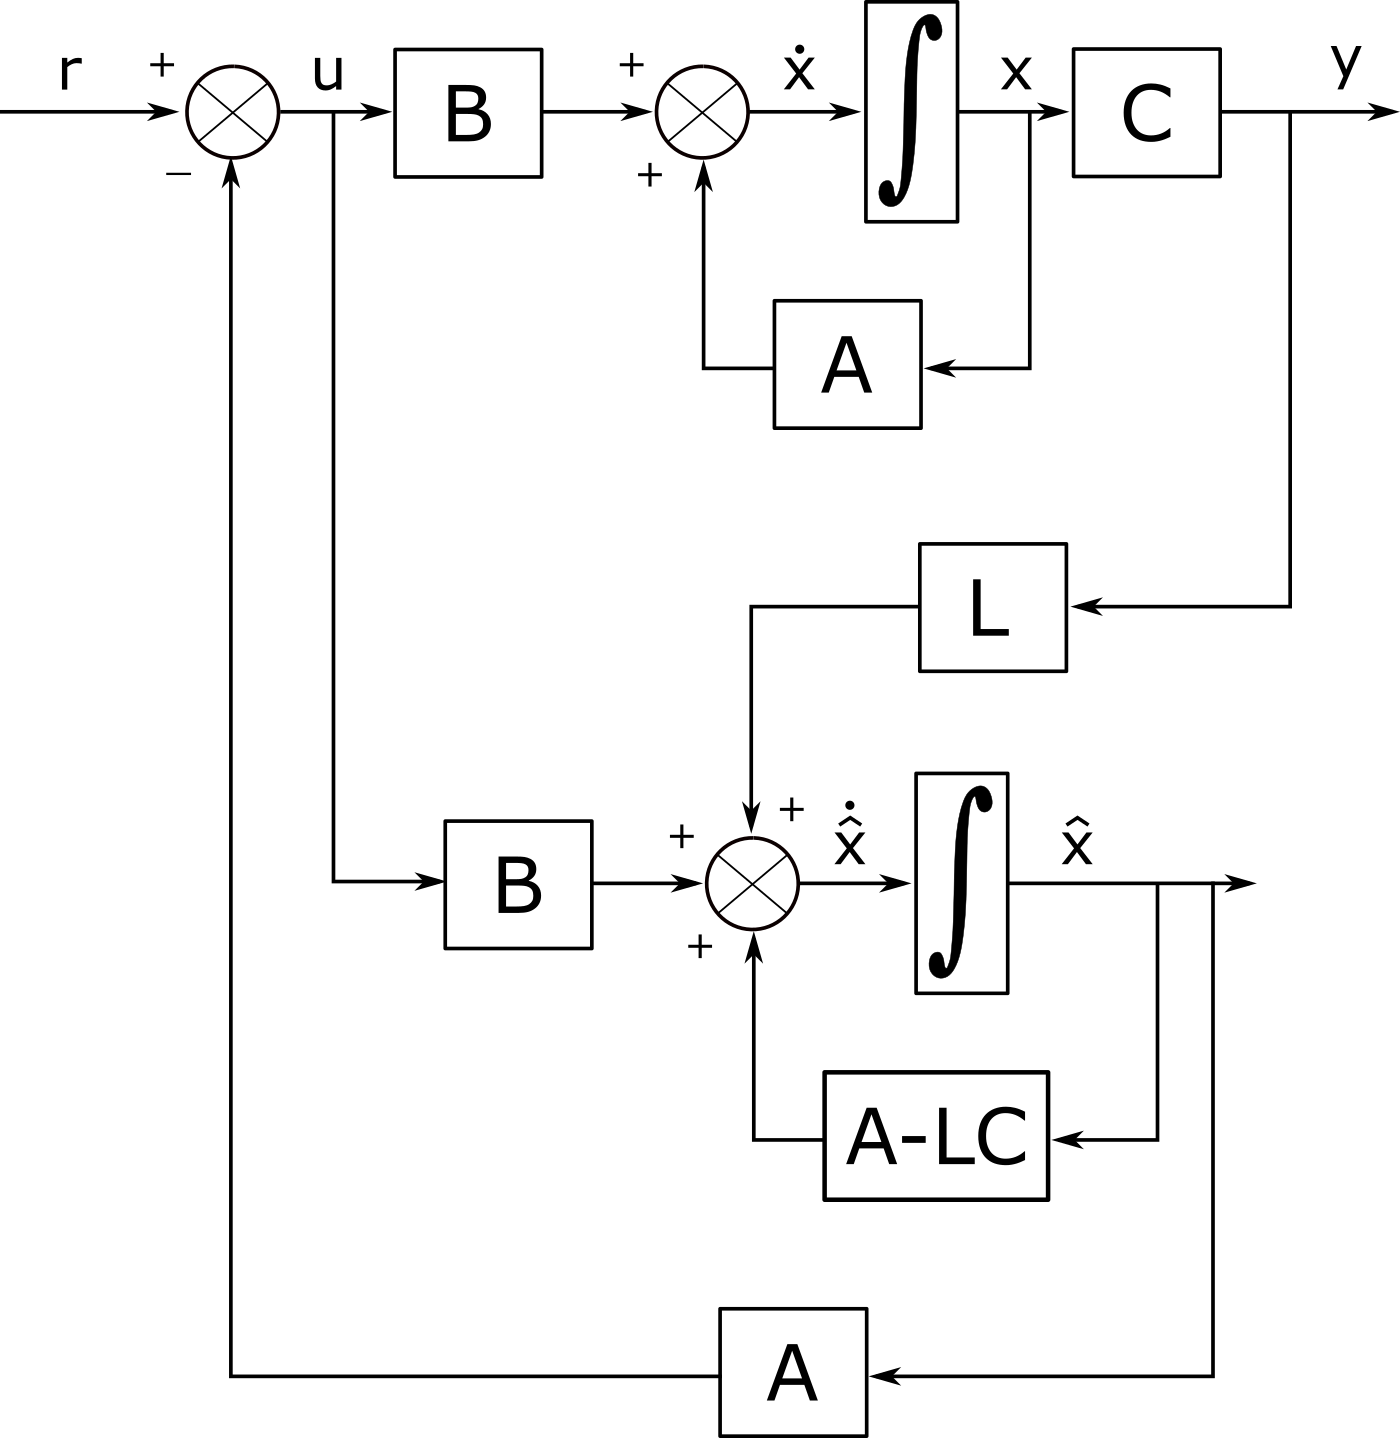
\includegraphics[scale=0.19]{Control de Sistemas Mecatronicos Figuras/11 Sistema con Observador Retroalimentado.png}
        \caption{Sistema retroalimentado basado en observación}
\end{figure}

Sustituyendo la retroalimentación del observador de estado \( u = r-k \hat{x} \) en el sistema (1) y en su observador se tiene que 
\[
    \begin{split}
        \dot{x} & = Ax + B(r-k\hat{x}) \\
        & = Ax - Bk\hat{x} + Br \\ 
        \dot{\hat{x}} & = A\hat{x} + B(r-k\hat{x}) + L(y-C\hat{x}) \\
        & = A\hat{x} - Bk\hat{x} + Br + L(Cx-C\hat{x}) \\
        & = A\hat{x} - Bk\hat{x} + Br + LCx - LC\hat{x} \\
        & = LCx + (A - BK - LC)\hat{x} +Br
    \end{split}
\]

entonces se puede escribir un solo sistema de la siguiente forma
\[
    \begin{bmatrix}
        \dot{x} \\ \dot{\hat{x}}
    \end{bmatrix} =
    \begin{bmatrix}
        A & -Bk \\
        LC & A-Bk-LC 
    \end{bmatrix}
    \begin{bmatrix}
        x \\ \hat{x}
    \end{bmatrix} +
    \begin{bmatrix}
        B \\ B
    \end{bmatrix} r
\]

%Regulación de sistemas lineales
\subsection{Regulación de sistemas lineales}
Sea el sistema
\[
    (1)
    \left\{
        \begin{array}{lll}
            \dot{x}(t) = Ax(t) + Bu(t)\\
            y(t) = Cx(t)
        \end{array}
    \right.
\]

Es posible convertirlo a una función de transferencia usando la transformada de Laplace
\[
    \begin{split}
        sx(s) & = Ax(s) + Bu(s)\\
        sx(s) - Ax(s) & = Bu(s)\\
        (sI-A)x(s) & = Bu(s)\\
        x(s) & = (sI-A)^{-1}Bu(s)\\
    \end{split}
\]

Sustituyendo en la salida del sistema (1)
\[
    \begin{split}
        y(s) & = Cx(s) \\
        y(s) & = C(sI-A)^{-1}Bu(s) \\
        \frac{y(s)}{u(s)} & = C(sI-A)^{-1}B
    \end{split}
\]

También se puede describir el sistema (1) con una función de transferencia obtenida a partir de un sistema de entradas-salidas 
\[
    \begin{split}
        y^{n}(t) + a_{1}y^{n-1}(t) + \ldots + a_{n}y(t) & = b_{1}u^{n-1}(t) + \ldots + b_{n}u(t) \\
        \mathcal{L} \{ y^{n}(t) + a_{1}y^{n-1}(t) + \ldots + a_{n}y(t) \} & = \mathcal{L} \{ b_{1}u^{n-1}(t) + \ldots + b_{n}u(t) \}\\
        y(s)s^{n} + a_{1}y(s)s^{n-1} + \ldots + a_{n}y(s) & = b_{1}u(s)s^{n-1} + \ldots + b_{n}u(s)\\
        y(s) (s^{n} + a_{1}s^{n-1} +\ldots + a_{n} ) & = u(s) (b_{1}s^{n-1} + \ldots + b_{n})
    \end{split}
\]

Se escribe la función de transferencia como 
\[
    g(s) = \frac{y(s)}{u(s)} = \frac{ b_{1}s^{n-1} + \ldots + b_{n} }{ s^{n} + a_{1}s^{n-1} +\ldots + a_{n} }
\]

Por lo tanto
\[
    g(s) = \frac{y(s)}{u(s)} = \frac{ b_{1}s^{n-1} + \ldots + b_{n} }{ s^{n} + a_{1}s^{n-1} +\ldots + a_{n} } = C(sI-A)^{-1}B
\]

También es posible escribir la función de transferencia a partir de los polos \( \mu_{1}, \mu_{2}, \ldots, \mu_{n} \) y los ceros \( q_{1}, q_{2}, \ldots, q_{m} \)
\[
    G(s) = \frac{(s-q_{1}) (s-q_{2}) \ldots (s-q_{m})}{(s-\mu_{1}) (s-\mu_{2}) \ldots (s-\mu_{n})} \;\; donde \;\; m < n
\]

Cuando \( r(t) = 0 \), es decir, no hay entradas, el sistema solo depende de los polos (respuesta natural), sin embargo, cuando la \( r(t) \not = 0 \) los ceros también participan en la respuesta del sistema.

%Regulación de sistemas lineales: caso 1
\subsection{Regulación de sistemas lineales: caso 1}

Cuando no hay integrador en la planta, es decir todos los polos son distintos de cero, el sistema en lazo cerrado no alcanza la referencia, por ello Se añade una ganancia en la referencia.
Considerando el sistema en lazo cerrado
\[
    (1)
    \left\{
        \begin{array}{lll}
            \dot{x}(t) = (A-Bk)x(t) + B\underbrace{r(t)}_{u(t)}\\
            y(t) = Cx(t)
        \end{array}
    \right.
\]

considerando que el sistema (1) tiene inicialmente una ganancia de 1, es decir, la función de transferencia es
\[
    \frac{y(s)}{u(s)} = C(sI-(A-Bk))^{-1}B = 1
\]

Se le agrega una ganancia \( N \) tal que
\[
    \frac{y(s)}{u(s)N} = C(sI-(A-Bk))^{-1}B = \frac{1}{N}
\]

o bien
\[
    \frac{y(s)}{u(s)} = NC(sI-(A-Bk))^{-1}B = 1 \\
\]

Para una entrada \( r \) constante, en estado estacionario se tiene que 
\[
    \begin{split}
        \lim_{t \to \inf}(\frac{y(s)}{u(s)}) & = NC(A-Bk)^{-1}B = 1\\
        N & = \frac{1}{C(A-Bk)^{-1}B}
    \end{split}
\]

Usando la representación con polos y ceros
\[
    \begin{split}
        \lim_{t \to \inf}(\frac{y(s)}{u(s)}) & = N \frac{ b_{1}s^{n-1} + \ldots + b_{n} }{ s^{n} + a_{1}s^{n-1} +\ldots + a_{n} } = 1 \\
        N \frac{b_{n}}{a_{n}} & = 1 \\
        N & = \frac{a_{n}}{b_{n}}
    \end{split}
\]

Por lo tanto
\[
    N = \frac{1}{C(A-Bk)^{-1}B} = \frac{a_{n}}{b_{n}}
\]

Se consigue reducir el error de estado estacionario a cero, pero debido a que no tiene un integrador, el sistema no responde correctamente ante ruido.

%Regulación de sistemas lineales: caso 2
\subsection{Regulación de sistemas lineales: caso 2}

Cuando no hay integrador en la planta, y en lugar de usar solo una ganancia en la entrada, se propone un integrador de la siguiente forma

considere el sistema 
\[
    (1)
    \left\{
        \begin{array}{lll}
            \dot{x}(t) = Ax(t) + Bu(t)\\
            y(t) = Cx(t)
        \end{array}
    \right.
\]

Se define la entrada al sistema (1)
\[
    u = K_{I}\xi - kx
\]

Sustituye (2) en (1)
\[
    \begin{split}
        \dot{x} & = Ax + B(k_{I}\xi - kx) \\
        & = Ax + Bk_{I}\xi - Bkx \\
        & = (A-Bk)x + Bk_{I}\xi
    \end{split}
\]

Del integrador se puede ver que
\[
    \begin{split}
       \dot{\xi} & = r - y \\
       & = r - Cx \;\; (3) 
    \end{split}
\]

Usando (2) y (3) se puede formar el sistema en lazo cerrado
\[
    \begin{bmatrix}
        \dot{x} \\ \dot{\xi}
    \end{bmatrix} = 
    \begin{bmatrix}
        A-Bk & Bk_{I} \\
        -C & 0
    \end{bmatrix}
    \begin{bmatrix}
        x \\ \xi
    \end{bmatrix} + r
    \begin{bmatrix}
        0 \\ 1
    \end{bmatrix} \;\; (4)
\]

En estado estacionario la ecuación (4)
\[
    \begin{bmatrix}
        \lim_{t \to \infty}\dot{x}(t) \\
        \lim_{t \to \infty}\dot{\xi}(t)
    \end{bmatrix} = 
    \begin{bmatrix}
        A-Bk & Bk_{I} \\
        -C & 0
    \end{bmatrix}
    \begin{bmatrix}
        \lim_{t \to \infty}x(t) \\ 
        \lim_{t \to \infty}\xi(t)
    \end{bmatrix} + r
    \begin{bmatrix}
        0 \\ 1
    \end{bmatrix} \;\; (5)
\]

Haciendo (4) - (5)
\[
    \begin{bmatrix}
        \dot{x} - \lim_{t \to \infty}\dot{x}(t) \\
        \dot{\xi} - \lim_{t \to \infty}\dot{\xi}(t)
    \end{bmatrix} = 
    \begin{bmatrix}
        A-Bk & Bk_{I} \\
        -C & 0
    \end{bmatrix}
    \begin{bmatrix}
        x - \lim_{t \to \infty}x(t) \\ 
        \xi - \lim_{t \to \infty}\xi(t)
    \end{bmatrix} + r \;\; (6)
\]

Se define el error
\[
    \begin{split}
        e_{x} & = x - \lim_{t \to \infty} x(t) \\
        e_{\xi} & = \xi - \lim_{t \to \infty} \xi(t
    \end{split}
\]

Se reescribe el sistema (6)
\[
    \begin{bmatrix}
        \dot{e_{x}} \\
        \dot{e_{\xi}}
    \end{bmatrix} = 
    \begin{bmatrix}
        A-Bk & Bk_{I} \\
        -C & 0
    \end{bmatrix}
    \begin{bmatrix}
        e_{x} \\ 
        e_{\xi}
    \end{bmatrix}
\]

el sistema (6) se separa de la siguiente forma
\[
    \begin{split}
    \begin{bmatrix}
        \dot{e_{x}} \\
        \dot{e_{\xi}}
    \end{bmatrix} & = 
    \begin{bmatrix}
        A & 0 \\
        -C & 0
    \end{bmatrix}
    \begin{bmatrix}
        e_{x} \\ 
        e_{\xi}
    \end{bmatrix}
    + B
    \begin{bmatrix}
        -k & +k_{I}
    \end{bmatrix}
    \begin{bmatrix}
        e_{x} \\ 
        e_{\xi}
    \end{bmatrix} \\
    & =
    \begin{bmatrix}
        A & 0 \\
        -C & 0
    \end{bmatrix}
    \begin{bmatrix}
        e_{x} \\ 
        e_{\xi}
    \end{bmatrix}
    - B
    \underbrace{
    \begin{bmatrix}
        k & -k_{I}
    \end{bmatrix}}_{\tilde{k}}
    \begin{bmatrix}
        e_{x} \\ 
        e_{\xi}
    \end{bmatrix}
    \end{split}
\]

donde 
\[ 
    e_{u} = -ke_{x} + k_{I}e_{\xi} = -\tilde{k} \begin{bmatrix}
        e_{x} \\ e_{\xi}
    \end{bmatrix} 
\]

También se puede ver de (1) en estado estacionario
\[
    \lim_{t \to \infty} u(t) = k_{I}\lim_{t \to \infty}\xi(t) - k\lim_{t \to \infty}x(t) (7)
\]

Haciendo (7) - (1)
\[
    \begin{split}
        u - \lim_{t \to \infty} u(t) & = k_{I}\xi - k_{I}\lim_{t \to \infty}\xi(t) - kx + k\lim_{t \to \infty}x(t) \\
        & = k_{I}(\xi - \lim_{t \to \infty}\xi(t)) - k(x - \lim_{t \to \infty}x(t)) \\
        & = K_{I}e_{\xi} - ke_{x}
    \end{split}
\]

Reescribiendo (4)
\[
    \begin{bmatrix}
        \dot{x} \\ \dot{\xi}
    \end{bmatrix} = 
    \begin{bmatrix}
        A & 0 \\
        -C & 0
    \end{bmatrix}
    \begin{bmatrix}
        x \\ \xi
    \end{bmatrix} +
    \begin{bmatrix}
        B \\ 0
    \end{bmatrix}u + r
    \begin{bmatrix}
        0 \\ 1
    \end{bmatrix} \;\; (8)  
\]

En estado estacionario (8)
\[
    \begin{bmatrix}
        \lim_{t \to \infty} \dot{x(t)} \\ 
        \lim_{t \to \infty} \dot{\xi} (t)
    \end{bmatrix} = 
    \begin{bmatrix}
        A & 0 \\
        -C & 0
    \end{bmatrix}
    \begin{bmatrix}
        \lim_{t \to \infty} x(t) \\
        \lim_{t \to \infty} \xi (t)
    \end{bmatrix} +
    \begin{bmatrix}
        B \\ 0
    \end{bmatrix} \lim_{t \to \infty} u(t) + r
    \begin{bmatrix}
        0 \\ 1
    \end{bmatrix} \;\; (9)
\]

Haciendo (8) - (9)
\[
    \begin{bmatrix}
        \dot{e_{x}} \\ 
        \dot{e_{\xi}}
    \end{bmatrix} = 
    \underbrace
    {
    \begin{bmatrix}
        A & 0 \\
        -C & 0
    \end{bmatrix}
    }_{\Tilde{A}}
    \begin{bmatrix}
        e_{x} \\
        e_{\xi}
    \end{bmatrix} +
    \underbrace
    {
    \begin{bmatrix}
        B \\ 0
    \end{bmatrix}
    }_{\tilde{B}}
    e_{u} \;\; (10)
\]

Se define la variable de estado como
\[
    E = 
    \begin{bmatrix}
        e_{x} \\ e_{\xi}
    \end{bmatrix}
\]

El sistema (10)
\[
    \dot{E} = \tilde{A}E + \tilde{B}e_{u} \;\; (11)
\]

Sustituyendo \( E \) en la definición de \( e_{u} \)
\[
    e_{u} = -\tilde{k}E \;\; (12)
\]

Sustituyendo (12) en (11)
\[
    \begin{split}
        \dot{E} & = \tilde{A}E + \tilde{B}(-\tilde{k}E) \\ 
        & = \tilde{A}E - \tilde{B}\tilde{k}E \\
        & = (\tilde{A} - \tilde{B}\tilde{k})E
    \end{split}
\]

Se resuelve como un problema de asignación de polos para la matriz \( \tilde{A} - \tilde{B}\tilde{k} \)

%Regulación de sistemas lineales: caso 3
\subsection{Regulación de sistemas lineales: caso 3}

La planta tiene un integrador, es decir, un polo en el origen

\begin{figure}[h!]
    \centering
        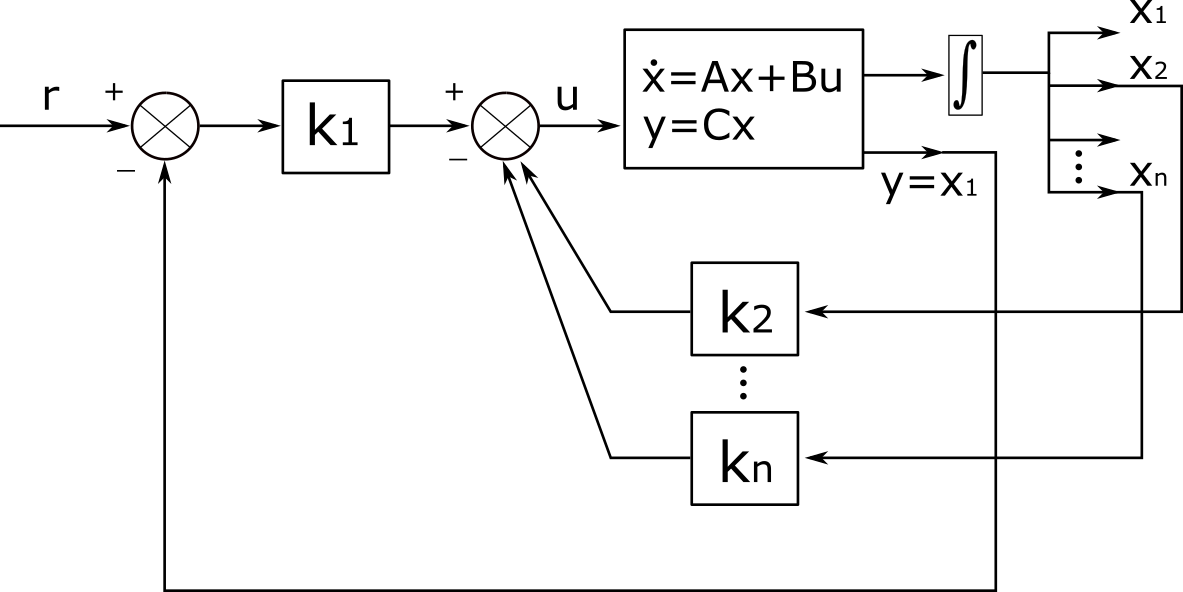
\includegraphics[scale=0.17]{Control de Sistemas Mecatronicos Figuras/16 Con integrador en la Planta.png}
        \caption{Sistema con integrador en la planta}
\end{figure}

Sea el sistema 
\[
    (1)
    \left\{
        \begin{array}{lll}
            \dot{x}(t) = Ax(t) + Bu(t) \\
            y(t) = Cx(t)
        \end{array}
    \right.
\]

La entrada del sistema es
\[
    \begin{split}
        u & = k_{1}(r - x_{1}) - k_{2}x_{2} - k_{3}x_{3} - \ldots - k_{n}x_{n} \\
        & = k_{1}r - k_{1}x_{1} - k_{2}x_{2} - k_{3}x_{3} - \ldots - k_{n}x_{n} \\
        & = k_{1}r - 
        \begin{bmatrix}
            k_{1} & k_{2} & \ldots & k_{n}
        \end{bmatrix}
        \begin{bmatrix}
            x_{1} \\ x_{2} \\ \vdots \\ x_{n}
        \end{bmatrix} \\
        & = k_{1}r - kx
    \end{split}
\]

\begin{figure}[h!]
    \centering
        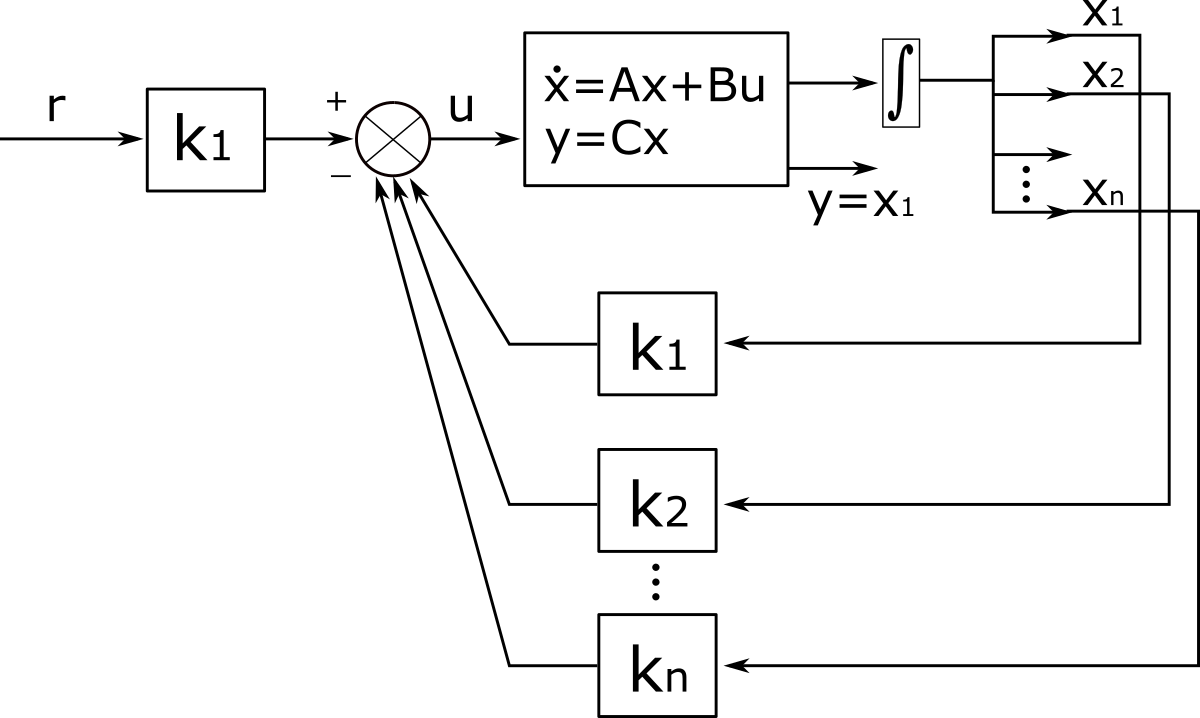
\includegraphics[scale=0.19]{Control de Sistemas Mecatronicos Figuras/17 Con integrador en la Planta.png}
        \caption{Sistema con integrador en la planta}
\end{figure}

Sustituyendo (2) en (1)
\[
    \begin{split}
        \dot{x} & = Ax + B(k_{1}r - kx) \\
        & = Ax + Bk_{1}r - Bkx \\
        & = (A-Bk)x + Bk_{1}r
    \end{split}
\]

El problema de regulación se resuelve como un problema de ubicación de polos para la matriz \( A-Bk \)

%Criterios para asignación de polos en lazo cerrado
\subsection{Criterios para asignación de polos en lazo cerrado}

Sea el sistema
\[(1)
    \left\{
        \begin{array}{lll}
            \dot{x}(t) = Ax(t) + Bu(t) \\
            y(t) = Cx(t)
        \end{array}
    \right.
\]

hay dos casos al momento de obtener la función de transferencia

\begin{itemize}
    \item a) Sin ceros
    \[
        \frac{x(s)}{y(s)} = \frac{b}{s^{n} + \tilde{a}_{1}s^{n-1} + \ldots + \tilde{a}_{n}} = \frac{b}{(s-\mu_{1})(s-\mu_{2})\ldots(s-\mu_{n})}
    \]
    \item b) Con ceros y polos
    \[
        \frac{x(s)}{y(s)} = \frac{(s-q_{1}) (s-q_{2}) \ldots (s-q_{m})}{(s-\mu_{1})(s-\mu_{2})\ldots(s-\mu_{n})} \;\; \text{con \( m < n \)}
    \]
    
\end{itemize}

La función de transferencia se aproxima a un sistema de segundo orden, de la forma
\[
    \frac{y(s)}{x(s)} = \frac{W_{n}}{s^{2} +2 \xi W_{n}s + W_{n}^{2} } \;\; (2)
\]

Donde 
\[
    \begin{split}
        \xi & : \text{amortiguamiento} \\
        W_{n} & : \text{frecuencia natural}
    \end{split}
\]

\begin{figure}[h!]
    \centering
        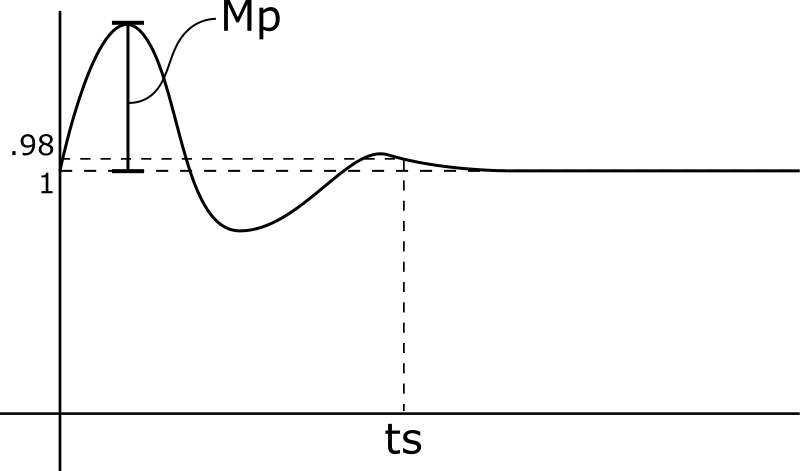
\includegraphics[scale=0.25]{Control de Sistemas Mecatronicos Figuras/18 Sistema de Segundo Orden.png}
        \caption{Sistema de segundo orden}
\end{figure}

Entonces se define el máximo sobre impulso
\[
    M_{p} = e^{^{- \xi \pi}/_{\sqrt{1 - \xi^{2}}}}
\]

Tiempo de asentamiento: tiempo para mantenerse alrededor del valor final
\[
    \begin{split}
        t_{s} = \frac{4}{\xi W_{n}} \;\; \text{Criterio del 2\%} \\
        t_{s} = \frac{3}{\xi W_{n}} \;\; \text{Criterio del 5\%}
    \end{split}
\]

La ecuación (2) se resuelve 
\[
    \text{polos dominantes} < S_{1,2} = -\xi W_{n} \pm W_{n}(\sqrt{\xi^{2} - 1})
\]

Polos no dominantes: deben de estar mas alejados de los dominantes, al menos 5 veces en valor absoluto del polo dominante

Para el caso b) eliminar los ceros con los polos, tal que
\[
    \mu_{3} \approx q_{1}, \mu_{4} \approx q_{2}, \ldots,
     \mu_{n+m} \approx q_{m} 
\]

%Estabilidad de Lyapunov
\subsection{Estabilidad de Lyapunov}

Método 1 directo \\
Requiere de la solución del sistema

\parskip .1in
Método 2 indirecto \\
No requiere solución del sistema, se basa en la dinámica del sistema

Definición (función definida positiva)
Una función escalar \( V(x) \) es definida positiva si
\[
    \begin{split}
        1) & \;\; V(0) = 0 \\
        2) & \;\; V(x) > 0 \text{  para todo \( x \not = 0 \)}
    \end{split}
\]

Definición (forma cuadrática)\\
Sea una matriz \( p > 0 \) y sea simétrica \( P = P^{T} \)
Con \( V(x) = x^{T}Px > 0 \)
Se tiene la desigualdad de Rayleight
\[
    \begin{split}
        \lambda_{min}(P) ||x||^{2} \leq & V(x) = x^{T}Px \leq \lambda_{max} (P) ||x||^{2} \\
        \lambda_{min}(I)||x||^{2} \leq & V(x) \leq \lambda(I) ||x^{*}||^{2}
    \end{split}
\]

Sea el sistema
\[
    \begin{split}
        & \dot{x}(t) = f(x)\\
        & x(0) = x_{0}
    \end{split}
\]

donde \( x \in R^{n} \) es el vector de estado y \( f: R^{n} \to R^{n}\)

Definición  (punto de equilibrio)
Un punto de equilibrio es aquel que satisface \( f(x^{*}) = 0 \)
\begin{itemize}
    \item a) Tiene un punto de equilibrio: 
    \[
        x^{*} = 0 \text{  Si A es invertible}
    \]
    \item b) Tiene un numero infinito de puntos de equilibrio, si A no es invertible
\end{itemize}

Segundo método de Lyapunov

Sea el sistema
\[
    \begin{split}
        & \dot{x}(t) = f(x)\\
        & f(0) = 0
    \end{split}
\]

Si existe una función \( V(x) \) tal que
\[
    \left\{
        \begin{array}{lll}
            (1) V(x) > 0\\
            (2) \dot{V}(x) \big |_{(x)} < 0
        \end{array}
    \right.
\]
entonces el punto de equilibrio es asintoticamente estable.

Sea el sistema \((1) \;\; \dot{x} = Ax \) determinar las condiciones de estabilidad en el sentido de Lyapunov
\begin{itemize}
    \item 1) 
    \[
        V(x) = x^{T}Px, \;\;\; P = P^{T}, \;\;\; P > 0
    \]
    
    \item 2) 
    \[
        \begin{split}
            \dot{V}(x) & = \dot{x}Px + x^{T}P\dot{x} \;\;\; \text{\;\;\; \;\;\(\dot{x}^{T} = (Ax)^{T} = x^{T}A^{T}\) }\\
            & = x^{T}A^{T}Px + x^{T}P\dot{x} \\
            & = x^{T}(A^{T}P + PA)x \;\;\; \text{  Sea \( Q > 0\) \( A^{T}P + PA = -Q\)} \\
            & = -x^{T}Qx
        \end{split}
    \]
\end{itemize}

%UNIDAD III
\section{UNIDAD III Introducción a los sistemas discretos}

Un sistema en tiempo discreto se define en función de un periodo de muestreo \( T \) y un instante de muestreo \( k \)
\[
    x((x+1)k) = f(k,x(k), T)
\]

Si \( T \) es constante
\[
    x(k+1) = f(k, x(k))
\]

\begin{figure}[h!]
    \centering
        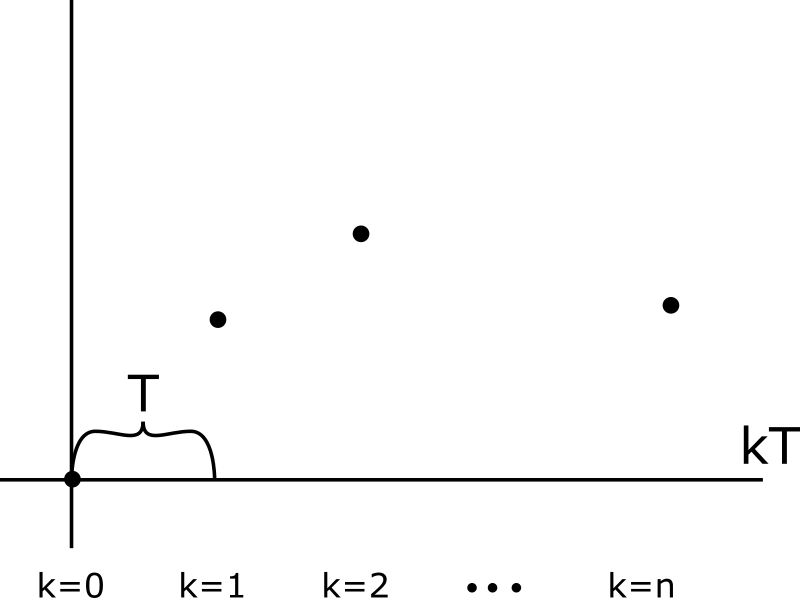
\includegraphics[scale=0.30]{Control de Sistemas Mecatronicos Figuras/19 Sistema en Tiempo Discreto.png}
        \caption{Sistemas en tiempo discreto}
\end{figure}

Las raíces del polinomio característico define la estabilidad del sistema.

Si todas las raíces tienen magnitud menor o igual que 1, el sistema es estable
\[
    |\mu_{i}| \leq 1
\]

%Forma canónica controlable
\subsection{Forma canónica controlable}

considere la representación entrada-salida 
\[
    (1) \;\;
    y(k) + a_{1}y(k-1) + \ldots + a_{n}y(k-n) = b_{1}u(k-1) + \ldots + b_{n}u(k-n)
\]  

Aplicando transformada Z a (1)
\[
    Y(z) + a_{1}z^{-1}Y(z) + \ldots + a_{n}z^{-n}Y(z) = b_{1}z^{-1}U(z) + \ldots + b_{n}z^{-n}U(z)
\]

Se obtiene la función de transferencia
\[
    \begin{split}
        \frac{Y(z)}{U(z)} & = \frac{b_{1}z^{-1} + b_{2}z^{-2} + \ldots + b_{n}z^{-n}}{1 + a_{1}z^{-1} + a_{2}z^{-2} + \ldots + a_{n}z^{-n}} \\ \;\; (2)
        & = \frac{b_{1}z^{n-1} + b_{2}z^{n-2} + \ldots + b_{n}}{z^{n} + a_{1}z^{n-1} + a_{2}z^{n-2} + \ldots + a_{n}} 
    \end{split}
\]

De (2)
\[
    \begin{split}
        & \frac{Y(z)}{b_{1}z^{-1} + b_{2}z^{-2} + \ldots + b_{n}z^{-n}} = \frac{U(z)}{1 + a_{1}z^{-1} + a_{2}z^{-2} + \ldots + a_{n}z^{-n}} = Q(z) \\
        & U(z) = Q(z) + a_{1}z^{-1}Q(z) + a_{2}z^{-2}Q(z) + \ldots + a_{n}z^{-n}Q(z) \\
        & (3)
        \left\{
            \begin{array}{lll}
                Q(z) = - a_{1}z^{-1}Q(z) - a_{2}z^{-2}Q(z) - \ldots - a_{n}z^{-n}Q(z) + U(z) \\
                Y(z) = b_{1}z^{-1}Q(z) + b_{2}z^{-2}Q(z) + \ldots + b_{n}z^{-n}Q(z)
            \end{array}
        \right.
        \end{split}
\]

A partir de (3) se definen las variables de estado
\[
    (4)\;\; X(z) = 
    \begin{bmatrix}
        X_{1}(z) \\
        X_{2}(z) \\
        \vdots \\
        X_{n-1}(z) \\
        X_{n}(z)
    \end{bmatrix} =
    \begin{bmatrix}
        z^{-n} \\
        z^{-n+1} \\
        \vdots \\
        z^{-2} \\
        z^{-1}
    \end{bmatrix} Q(z) \\
\]

Haciendo el cambio de variables en (3)
\[ (5)
    \left\{
        \begin{array}{lll}
            Q(z) = -a_{n}X_{1} - a_{n-1}X_{2} - \ldots - a_{2}X_{n-1}(z) - a_{1}X_{n}(z) + U(z) \\
            Y(z) = b_{1}X_{n}(z) + b_{2}x_{n-1}(z) + \ldots + b_{n}X_{1}(z) \ =
            [b_{n} \; b_{n-1} \; \ldots \; b_{1}] X(z)
        \end{array}
    \right.
\]

Multiplicamos (4) por z

\[ (6)
    \left\{
        \begin{array}{lll}
            zX_{1}(z) = z^{-n+1}Q(z) = X_{2}(z) \\
            zX_{2}(z) = z^{-n+2}Q(z) = X_{3}(z) \\
            \;\;\;\;\;\;\; \vdots \\
            zX_{n-1}(z) = z^{-1}Q(z) = X_{n}(z) \\
            zX_{n}(z) = Q(z)
        \end{array}
    \right.
\]

Se sustituye (4) en (5), considerando el ultimo termino de (6)
\[ (7)
    \left\{
        \begin{array}{lll}
            zX_{n}(z) = Q(z) = [-a_{n} \; -a_{n-1} \; \ldots \; -a_{1}]X(z) + U(z) \\
            Y(z) = [b_{n} \; b_{n-1} \; \ldots \; b_{1}] X(z)
        \end{array}
    \right.
\]

se aplica la transformada inversa a las variables de estado(4)
\[
    X(k) = 
    \begin{bmatrix}
        X_{1}(k) \\
        X_{2}(k) \\
        \vdots \\
        X_{n-1}(k) \\
        X_{n}(k)
    \end{bmatrix}
\]

Se aplica la transformada inversa a (6) y (7)
\[ (7)
    \left\{
        \begin{array}{lll}
            X_{1}(k+1) = X_{2}(k) \\
            X_{2}(k+1) = X_{3}(k) \\
            \;\;\;\;\;\;\; \vdots \\
            X_{n-1}(k+1) = X_{n}(k) \\
            X_{n}(k+1) = Q(k) = [-a_{n} \; -a_{n-1} \; \ldots \; -a_{1}]X(k) + U(k) \\
            y(k) = [b_{n} \; b_{n-1} \; \ldots \; b_{1}] X(k)
        \end{array}
    \right.
\]

se obtiene la forma canónica controlable de (7)
\[
    \begin{split}
        x(k+1) & = 
        \begin{bmatrix}
            0 & 1 & 0 & \cdots & 0 \\
            0 & 0 & 1 & \cdots & 0 \\
            \vdots & \vdots & \ddots & \ddots & \vdots \\
            0 & 0 & \ldots & 0 & 1 \\
            -a_{n} & -a_{n-1} & \cdots & -a_{2} & -a_{1}
        \end{bmatrix}x(k) +
        \begin{bmatrix}
            0 \\ 0 \\ 0 \\ \vdots \\ 1
        \end{bmatrix}u(k) \\
        y(k) & = 
        \begin{bmatrix}
            b_{n} & b_{n-1} & \ldots b_{2} & b_{1}    
        \end{bmatrix} X(k)
    \end{split}
\]

%Forma canónica observable
\subsection{Forma canónica observable}

Considere el sistema (1)
\[
    \begin{split}
        (1) \;\; & y(k) + a_{1}y(k-1) + a_{2}y(k-2) + \ldots + a_{n}y(k-n) \\
            & = b_{1}u(k-n) + b_{2}u(k-2) + \ldots + b_{n}u(k-n)
    \end{split}
\]

Aplicando transformada Z a la ecuación (1)
\[
    \begin{split}
        & Y(z) + a_{1}z^{-1}Y(Z) + a_{2}z^{-2}Y(z) + \ldots + a_{n}z^{-n}Y(z) \\
        & = b_{1}z^{-1}U(z) + b_{2}z^{-2}U(z) + \ldots + b_{n}z^{-n}U(z) \\
        & Y(z) = z^{-1}[b_{1}U(z)-a_{1}Y(z)] + z^{-2}[b_{2}U(z)-a_{2}Y(z)] + \ldots + \\
        & z^{-n+1}[b_{n-1}U(z)-a_{n-1}Y(z)] + \ldots + z^{-n}[b_{n}U(z)-a_{n}Y(z)] \\
        & Y(z) = z^{-1}[b_{1}U(z)-a_{1}Y(z)] + z^{-1}z^{-1}[b_{2}U(z)-a_{2}Y(z)] + \ldots + \\
        & z^{-n+1}[b_{n-1}U(z)-a_{n-1}Y(z)] + \ldots + z^{-n}[b_{n}U(z)-a_{n}Y(z)] \\
        (2) & Y(z) = z^{-1} [b_{1}U(z)-a_{1}Y(z) + z^{-1}\{b_{2}U(z)-a_{2}Y(z) + z^{-1}(b_{3}U(z)-a_{3}Y(z) + \ldots + \\
        & z^{-1}[b_{n-1}U(z)-a_{n-1}Y(z) + z^{-1}(b_{n}U(z)-a_{n}Y(z))]\ldots)\}]
    \end{split}
\]

Con \( Y(z) = x_{n}(z) \), a partir de (2) se definen las variables de estado
\[(3)
    \left\{
        \begin{array}{lll}
            X_{1}(z) = z^{-1}(b_{n}U(z)-a_{n}Y(z)) \\ 
            x_{2}(z) = z^{-1}(b_{n-1}U(z)-a_{n-1}Y(z)+X_{1}(z)) \\
            \;\;\;\;\;\;\;\;\;\; \vdots \\
            x_{n-1}(z) = z^{-1}(b_{2}U(z)-a_{2}Y(z) + X_{n-2}(z)) \\
            X_{n}(z) = z^{-1}(b_{1}U(z)-a_{1}X_{n}(z)+x_{n-1}(z))
        \end{array}
    \right.
\]

Se multiplica (3) por z y se agrega la salida del sistema
\[(4)
    \left\{
        \begin{array}{lll}
            zX_{1}(z) = b_{n}U(z)-a_{n}Y(z) \\ 
            zx_{2}(z) = b_{n-1}U(z)-a_{n-1}Y(z)+X_{1}(z) \\
            \;\;\;\;\;\;\;\;\;\; \vdots \\
            zx_{n-1}(z) = b_{2}U(z)-a_{2}Y(z) + X_{n-2}(z) \\
            zX_{n}(z) = b_{1}U(z)-a_{1}X_{n}(z)+x_{n-1}(z) \\
            Y(z) = x_{n}(z)
        \end{array}
    \right.
\]

Aplicando transformada inversa  a (4)
\[(5)
    \left\{
        \begin{array}{lll}
            X_{1}(k+1) = b_{n}u(k)-a_{n}y(k) \\ 
            X_{2}(k+1) = b_{n-1}u(k)-a_{n-1}y(k)+X_{1}(k) \\
            \;\;\;\;\;\;\;\;\;\; \vdots \\
            X_{n-1}(k+1) = b_{2}u(k)-a_{2}y(k) + X_{n-2}(k) \\
            X_{n}(k+1) = b_{1}u(k)-a_{1}X_{n}(k)+x_{n-1}(k) \\
            y(k) = X_{n}(k)
        \end{array}
    \right.
\]

A partir de (5) se obtiene la forma canónica observable
\[
    \begin{split}
        x(k+1) & = 
        \begin{bmatrix}
            0 & 0 & 0 & \cdots & -a_{n} \\
            1 & 0 & 0 & \cdots & -a_{n-1} \\
            \vdots & \vdots & \ddots & \ddots & \vdots \\
            0 & 0 & \ldots & 0 & -a_{2} \\
            0 & 0 & \cdots & 1 & -a_{1}
        \end{bmatrix}x(k) +
        \begin{bmatrix}
            b_{n} \\ b_{n-1} \\ \vdots \\ b_{2} \\ b_{1}
        \end{bmatrix}u(k) \\
        y(k) & = 
        \begin{bmatrix}
            0 & 0 & \ldots & 0 & 1    
        \end{bmatrix} X(k)
    \end{split}
\]

%Forma canónica diagonal
\subsection{Forma canónica diagonal}

Considere el sistema (1)
\[
    \begin{split}
        (1) \;\; & y(k) + a_{1}y(k-1) + a_{2}y(k-2) + \ldots + a_{n}y(k-n) \\
            & = b_{1}u(k-n) + b_{2}u(k-2) + \ldots + b_{n}u(k-n)
    \end{split}
\]

Se obtiene la función de transferencia 
\[
    \begin{split}
        \frac{ Y(z) }{ U(z) } & = \frac{ b_{1}z^{-1} + b_{2}z^{-2} + \ldots + b_{n}z^{-n} }{ 1 + a_{1}z^{-1} + a_{2}z^{-2} + \ldots + a_{n}z^{-n} } \frac{ z^{n} }{ z^{n} } \\ \;\;
        & = \frac{b_{1}z^{n-1} + b_{2}z^{n-2} + \ldots + b_{n}}{ z^{n} + a_{1}z^{n-1} + a_{2}z^{n-2} + \ldots + a_{n} } \\
        & = \frac{ b_{1}z^{n-1} + b_{2}z^{n-2} + \ldots + b_{n} }{ (s-q_{1})(s-q_{2}) \ldots (s-q_{n}) }
    \end{split}
\]

Sea \( q_{1}, q_{2}, \ldots, q_{n} \), raíces del polinomio P(z). Se asume que todas las raíces son distintas, entonces se define (2) en fracciones parciales
\[
    (3) \;\;
    \frac{ C_{1} }{ z - q_{1} }U(z) + \frac{ C_{2} }{ z-q_{2} }U(z) + \ldots + \frac{ C_{n} }{ z - q_{n} }U(z)
\]

Se definen las variables de estado de (3)
\[(4)
    \left\{
        \begin{array}{lll}
            X_{1}(z) = \frac{ 1 }{ z - q_{1} }U(z) \\ 
            x_{2}(z) = \frac{ 1 }{ z - q_{2} }U(z) \\
            \;\;\;\;\;\;\;\;\;\; \vdots \\
            X_{n}(z) = \frac{ 1 }{ z - q_{n} }
        \end{array}
    \right.
\]

Sustituyendo (4) en (3)
\[
    \begin{split}
        Y(z) & = X_{1}C_{1} + X_{2}C_{2} + \ldots + X_{n}C_{n} \\
        (5) \;\; Y(z) & = 
        \begin{bmatrix}
            C_{1} & C_{2} & \ldots & C_{n} 
        \end{bmatrix} X(z)
    \end{split}
\]

Si se toma una variable de estado
\[
    \begin{split}
        X_{1}(z) & = \frac{ 1 }{ z-q_{1} }U(z) \\
        X_{1}(z)(z-q_{1}) & = U(z) \\
        zX_{1}(z) - X_{1}(z)q_{1} & = U(z) \\
        zX_{1}(z) & = U(z) + X_{1}(z)q_{1}
    \end{split}
\]

Aplicando el mismo procedimiento a todas las variables de estado
\[(6)
    \left\{
        \begin{array}{lll}
            zX_{1}(z) & = U(z) + X_{1}(z)q_{1} \\ 
            zX_{2}(z) & = U(z) + X_{2}(z)q_{2} \\
            \;\;\;\;\;\;\;\;\;\; \vdots \\
            zX_{n}(z) & = U(z) + X_{n}(z)q_{n}
        \end{array}
    \right.
\]

Aplicando transformada inversa a (5) y (6)
\[(7)
    \left\{
        \begin{array}{lll}
            X_{1}(k+1) & = q_{1}X_{1}(k) + u(k) \\ 
            X_{2}(k+1) & = q_{2}X_{2}(k) + u(k) \\
            \;\;\;\;\;\;\;\;\;\; \vdots \\
            X_{n}(k+1) & = q_{n}X_{n}(k) + u(k) \\
            y(k) & = 
            \begin{bmatrix}
                C_{1} & C_{2} & \ldots & C_{n} 
            \end{bmatrix} X(k)
        \end{array}
    \right.
\]

A partir de (7) se obtiene la forma canónica diagonal
\[
    \begin{split}
        X(k+1) & = 
        \begin{bmatrix}
            q_{1} & 0 & \cdots & 0 \\
            0 & q_{2} & \cdots & 0 \\
            \vdots & \ddots & \ddots & \vdots \\
            0 & 0 & \cdots & q_{n}
        \end{bmatrix}X(k) +
        \begin{bmatrix}
            1 \\ 1 \\ \vdots \\ 1
        \end{bmatrix}u(k) \\
        y(k) & = 
        \begin{bmatrix}
            C_{1} & C_{2} & \ldots & C_{n}   
        \end{bmatrix} X(k)
    \end{split}
\]

%Solución de ecuaciones en espacio de estados
\subsection{Solución de ecuaciones en espacio de estados}

Considere el sistema
\[
    (1)
    \left\{
        \begin{array}{lll}
            x(k+1)= Ax(k) + Bu(k)\\
            y(k) = Cx(k)
        \end{array}
    \right.
\]
Con condición inicial \( x(0) = x_{0} \)

El problema consiste en determinar el vector de estado \( x(k) \) y la salida \( y(k) \)

Se aplica la transformada \( Z \) al sistema (1)
\[
    \begin{split}
        &\left\{
        \begin{array}{lll}
            \mathcal{Z} \{ x(k+1) \}= \mathcal{Z} \{ Ax(k) \} + \mathcal{Z} \{ Bu(k) \}\\
            \mathcal{Z} \{ y(k) \} = \mathcal{Z} \{ Cx(k) \}
        \end{array}
        \right. \\
        &\left\{
            \begin{array}{lll}
                zX(z) -zX(0) = AX(z) + BU(z) \\
                y(z) = CX(z)
            \end{array}
        \right. \\
        &\left\{
            \begin{array}{lll}
                zX(z) - AX(z) = zX(0) + BU(z) \\
                y(z) = CX(z)
            \end{array}
        \right. \\
        &\left\{
            \begin{array}{lll}
                (zI-A)X(z) = zX(0) + BU(z) \\
                y(z) = CX(z)
            \end{array}
        \right. \\
        (2) \;\; &\left\{
            \begin{array}{lll}
                X(z) = (zI-A)^{-1}zX(0) + (zI-A)^{-1}BU(z) \\
                y(z) = C(zI-A)^{-1}zX(0) + C(zI-A)^{-1}BU(z)
            \end{array}
        \right.
        \end{split}
\]

Para condiciones iniciales \( X(0) = 0 \)
\[
    \frac{Y(z)}{U(z)} = C(zI-A)^{-1}B 
    \left\}
            \begin{array}{lll}
                \text{Matriz de} \\
                \text{transferencia}
            \end{array}
    \right.
\]

Aplicando transformada inversa a (2)
\[
    \mathcal{Z}^{-1} \{ X(z) \} = x(k) = \mathcal{Z}^{-1} \{ (zI-A)^{-1}z \}x(0) + \mathcal{Z}^{-1} \{ (zI-A)^{-1}BU(z) \}
\]
\[
    y(k) = Cx(k) = 
    \underbrace{C \mathcal{Z}^{-1} \{ (zI-A)^{-1}z \}x(0)}_
    {
        \begin{scriptsize}
            \begin{matrix}
                \text{Solución homogénea}\\
                \text{natural}\\
            \end{matrix}
        \end{scriptsize}
    }+ 
    \underbrace{C \mathcal{Z}^{-1} \{ (zI-A)^{-1}BU(z) \}}_
    {
        \begin{scriptsize}
            \begin{matrix}
                \text{Solución particular}\\
                \text{forzada}\\
            \end{matrix}
        \end{scriptsize}
    }
\]

Se define la matriz de transición de estado
\[
    \mathcal{Z}^{-1} \{ (zI-A)^{-1} z \}
\]

%Discretización de ecuaciones en espacio de estado
\subsection{Discretización de ecuaciones en espacio de estado}

Sea el sistema
\[(1)
    \left\{
        \begin{array}{lll}
            \dot{x}(t) = Ax(t) + Bu(t) \\
            y(t) = Cx(t)
        \end{array}
    \right.
\]
con condición inicial \( x(0) = x_{0} \)

El problema de discretización consiste en obtener un sistema dinámico equivalente para el sistema (1) en tiempo discreto de la forma
\[
    \left\{
        \begin{array}{lll}
            \dot{x}(k+1) = Ax(k) + Bu(k) \\
            y(k) = Cx(k)
        \end{array}
    \right.
\]

donde
\[
    \left\{
        \begin{array}{lll}
            \dot{x}((k+1)T) = Ax(kT) + Bu(kT) \\
            y(kT) = Cx(kT)
        \end{array}
    \right.
\]

\begin{figure}[ht]
    \centering
        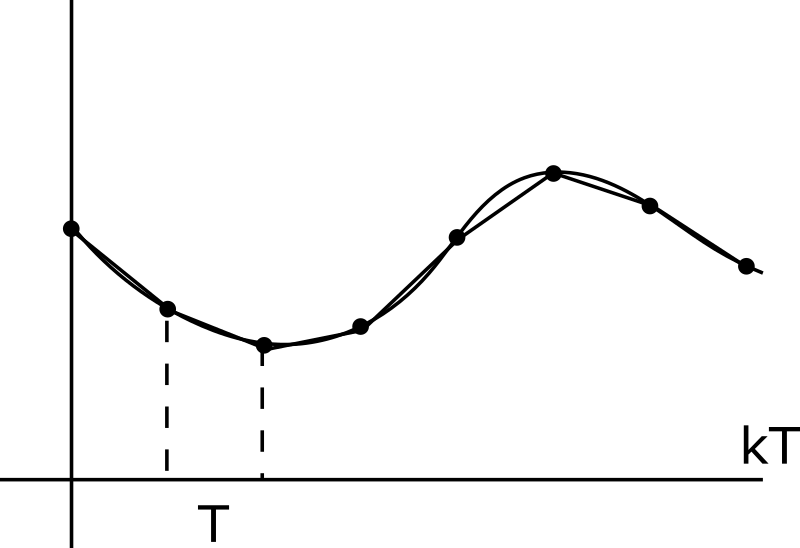
\includegraphics[scale=0.30]{Control de Sistemas Mecatronicos Figuras/20 Continuo a Discreto.png}
        \caption{Continuo a discreto}
\end{figure}

La solución de la ecuación (1) es 
\[
    (2) \;\; x(t) = e^{At}x(0) + \int_{0}^{t}e^{ A(t-\tau) }Bu(\tau)d\tau
\]

Haciendo \( t = (k+1)T \) en la ecuación (2)
\[
    (3) \;\; x((k+1)T) = e^{ A(k+1)T }x(0) + e^{ A(k+1)T } \int_{0}^{ (k+1)T } e^{ -A\tau }Bu(\tau)d\tau
\]

Haciendo \( t = kT \) en la ecuación (2)
\[
    (4) \;\; x(kT) = e^{ AkT }x(0) + e^{ AkT }\int_{0}^{kT} e^{ -A\tau }Bu(\tau)d\tau
\]

Multiplicar (4) por \( e^{AT} \)
\[
    \begin{split}
        (5) \;\; e^{ AT }x(kT) & = e^{ AT }e^{AkT}x(0) + e^{ AT }e^{AkT}\int_{0}^{kT} e^{ -A\tau }Bu(\tau)d\tau \\
        & = e^{A(k+1)T}x(0) + e^{A(k+1)T}\int_{0}^{kT} e^{-A\tau}Bu(\tau)d\tau
    \end{split}
\]

Restarle (5) a (3)
\[
    \begin{split}
        x((k+1)T) - e^{AT}x(kT) & = e^{A(k+1)T} \int_{0}^{(k+1)T} e^{-A \tau}Bu(\tau)d\tau - \\ 
        & e^{A(k+1)T}\int_{0}^{kT}e^{-A \tau}Bu(\tau)d\tau \\
        & = e^{A(k+1)T}\int_{kT}^{(k+1)T}e^{-A \tau}Bu(\tau)d\tau \\
        x((k+1)T) & = e^{AT}x(kT) + e^{A(k+1)T}\int_{kT}^{(k+1)T}e^{-A \tau}Bu(\tau)d\tau 
    \end{split}
\]

Se asume \( u(t) \) es constante para \( kT \leq t \leq (k+1)T \)
\[
    \begin{split}
        (6) \;\; x((k+1)T) & = e^{AT}x(kT) + e^{A(k+1)T}\int_{kT}^{(k+1)T}e^{-A \tau}d\tau Bu(kT)  
    \end{split}
\]

Se puede ver que \( e^{A(k+1)T} \int_{kT}^{(k+1)T} e^{-A\tau} d\tau \) se puede resolver por cambio de variable 
\[
    \begin{split}
        u & = -A\tau \\
        du & = -Ad\tau \\
        -A^{-1}du & = d\tau \\
        \text{con limites} \\
        u_{kT} & = -AkT \\
        u_{(k+1)T} & = -A(k+1)T
    \end{split}
\]
\[
    \begin{split}
        e^{A(k+1)T} \int_{kT}^{(k+1)T} e^{-A\tau} d\tau & = e^{A(k+1)T} \int_{-AkT}^{-A(k+1)T} e^{u}(-A^{-1})du \\
        & = e^{A(k+1)T} \big|_{-AkT}^{-A(k+1)T} e^{u}(-A^{-1}) \\
        & = e^{A(k+1)T} [e^{-A(k+1)T} - e^{-AkT}] (-A^{-1}) \\
        & = [e^{0} - e^{AT}](-A^{-1}) \\
        & = [e^{AT} - I]A^{-1}
    \end{split}
\]

El resultado es el mismo si se aplica la integral por un periodo \( T \), usando el mismo cambio de variable, pero cambiando los limites a 
\[
    \begin{split}
        u_{T} & = -AT \\
        u_{0} & = 0
    \end{split}
\]
\[
    \begin{split}
        e^{ AT } \int_{0}^{T} e^{ -A\tau } d\tau & = e^{ AT } \int_{0}^{ -AT } e^{ u }(-A^{-1})du \\
        & = e^{ AT } \big|_{0}^{-AT} e^{u}(-A^{-1}) \\
        & = e^{ AT } [ e^{-AT} - e^{0} ] (-A^{-1}) \\
        & = [ e^{0} - e^{AT} ](-A^{-1}) \\
        & = [ e^{ AT } - I ]A^{-1}
    \end{split}
\]

por lo tanto, es posible sustituir la integral de (6)
\[
    \begin{split}
        (6) \;\; x((k+1)T) & = e^{ AT }x(kT) + e^{ AT } \int_{0}^{T} e^{ -A\tau } d\tau Bu(kT) \\
        & = e^{ AT }x(kT) + \int_{0}^{T} e^{ A(T-\tau) } d\tau Bu(kT)
    \end{split}
\]

se realiza un cambio de variable 
\[ 
    \begin{split}
        \lambda & = T - \tau \\
        d\lambda & = -d\tau \\
        \text{con limites} \\
        \lambda_{T} & = 0 \\
        \lambda_{0} & = T
    \end{split} 
\]
\[
    \begin{split}
        \;\; x((k+1)T) & = e^{ AT }x(kT) - \int_{T}^{0} e^{A\lambda} d\lambda Bu(kT) \\
        & = e^{ AT }x(kT) + \int_{0}^{T} e^{ A\lambda } d\lambda Bu(kT)
    \end{split}
\]

Entonces se definen
\[
    \begin{split}
        A(t) & = e^{ AT } \\
        B(t) & = \big( \int_{0}^{T} e^{ A\lambda } d\lambda \big) B
    \end{split}
\]

\end{document}
